\documentclass[12pt]{article}
\usepackage[authoryear]{natbib}

\usepackage{natbib}%Referencias coloridas
\usepackage[colorlinks, breaklinks, citecolor=blue,urlcolor=blue]{hyperref}%Referencias coloridas

\usepackage{graphicx}
\usepackage{amssymb}
\usepackage{amsmath}
\usepackage{times}
\usepackage{bm}
\usepackage{listings}
\usepackage[svgnames]{xcolor}
\usepackage{float}

\PassOptionsToPackage{hyphens}{url}\usepackage{hyperref}

\lstset{language=python,
	basicstyle=\small\ttfamily,
	deletekeywords={remotes},
	keywordstyle=\color{blue}
}

%%%%%%%%%%%%%%%%%%%%%%%%%%%%%%%%%%%%%%%%%%%%%%%%%%%%%%%%%%%%
\setlength{\textwidth}{27pc}
\setlength{\hoffset}{-19mm} \setlength{\textwidth}{170mm}
\setlength{\textheight}{235mm} \setlength{\voffset}{-15mm}
\renewcommand\baselinestretch{1.2}
%%%%%%%%%%%%%%%%%%%%%%%%%%%%%%%%%%%%%%%%%%%%%%%%%%%%%%%%%%%%

%%% Newcommand
\newcommand{\Es}{{\rm E}}
\newcommand{\e}{{\rm e}}
\newcommand{\Reais}{\mathbb{R}}
\newcommand{\de}{{\rm d}}

\newcommand{\Cn}{{\bf C}}
\newcommand{\ele}{{\it l}}
\newcommand{\dn}{{\bf d}}
\newcommand{\Dn}{{\bf D}}
\newcommand{\xn}{{\bf x}}
\newcommand{\Un}{{\bf U}}
\newcommand{\Kn}{{\bf K}}
\newcommand{\Xn}{{\bf X}}
\newcommand{\Vn}{{\bf V}}
\newcommand{\bn}{{\bf b}}
\newcommand{\an}{{\bf a}}
\newcommand{\cn}{{\bf c}}
\newcommand{\en}{{\bf e}}
\newcommand{\Bn}{{\bf B}}
\newcommand{\An}{{\bf A}}
\newcommand{\yn}{{\bf y}}
\newcommand{\Yn}{{\bf Y}}
\newcommand{\Zn}{{\bf Z}}
\newcommand{\zn}{{\bf z}}
\newcommand{\Hn}{{\bf H}}
\newcommand{\Gn}{{\bf G}}
\newcommand{\Mn}{{\bf M}}
\newcommand{\fn}{{\bf f}}
\newcommand{\hn}{{\bf h}}
\newcommand{\In}{{\bf I}}
\newcommand{\Fn}{{\bf F}}
\newcommand{\En}{{\bf E}}
\newcommand{\Jn}{{\bf J}}
\newcommand{\Ln}{{\bf L}}
\newcommand{\rn}{{\bf r}}
\newcommand{\un}{{\bf u}}
\newcommand{\Rn}{{\bf R}}
\newcommand{\Sn}{{\bf S}}
\newcommand{\Wn}{{\bf W}}
\newcommand{\wn}{{\bf w}}
\newcommand{\vn}{{\bf v}}
\newcommand{\alpn}{{\mbox{\boldmath $\alpha$}}}
\newcommand{\phn}{{\mbox{\boldmath $\phi$}}}
\newcommand{\epsiln}{{\mbox{\boldmath $\epsilon$}}}
\newcommand{\rhn}{{\mbox{\boldmath $\rho$}}}
\newcommand{\betn}{{\mbox{\boldmath $\beta$}}}
\newcommand{\deltn}{{\mbox{\boldmath $\delta$}}}
\newcommand{\sigmn}{{\mbox{\boldmath $\beta$}}}
\newcommand{\gamn}{{\mbox{\boldmath $\gamma$}}}
\newcommand{\Gamn}{{\mbox{\boldmath $\Gamma$}}}
\newcommand{\lamn}{{\mbox{\boldmath $\lambda$}}}
\newcommand{\Lamn}{{\mbox{\boldmath $\Lambda$}}}
\newcommand{\mun}{{\mbox{\boldmath $\mu$}}}
\newcommand{\etn}{{\mbox{\boldmath $\eta$}}}
\newcommand{\tetn}{{\mbox{\boldmath $\theta$}}}
\newcommand{\Tetn}{{\mbox{\boldmath $\Theta$}}}
\newcommand{\Deltn}{{\mbox{\boldmath $\Delta$}}}
\newcommand{\Phin}{{\mbox{\boldmath $\Phi$}}}
\newcommand{\Psin}{{\mbox{\boldmath $\Psi$}}}
\newcommand{\psin}{{\mbox{\boldmath $\psi$}}}
\newcommand{\Upin}{{\mbox{\boldmath $\Upsilon$}}}
\newcommand{\upin}{{\mbox{\boldmath $\upsilon$}}}
\newcommand{\Sign}{{\mbox{\boldmath $\Sigma$}}}
\newcommand{\Omegn}{{\mbox{\boldmath $\Omega$}}}
\newcommand{\omegn}{{\mbox{\boldmath $\omega$}}}
\newcommand{\eln}{{\mbox{\boldmath $\ell$}}}
\newcommand{\taun}{{\mbox{\boldmath $\tau$}}}
\newcommand{\bet}{\boldmath $\beta$ \unboldmath}%texto
\newcommand{\al}{\boldmath $\alpha$ \unboldmath}%texto
\newcommand{\teta}{\boldmath $\theta$ \unboldmath}
\newcommand{\mi}{\boldmath $\mu$ \unboldmath}
\newcommand{\et}{\boldmath $\eta$ \unboldmath}
\newcommand{\bbeta}{\textrm{\bet}}%equac\~{a}o
\newcommand{\ale}{\textrm{\al}}%equac\~{a}o
\newcommand{\tet}{\textrm{\teta}}
\newcommand{\mie}{\textrm{\mi}}
\newcommand{\eti}{\textrm{\et}}

\hyphenation{para-meters cons-truct cons-tants}
\usepackage{enumerate}


\title{A competitive family to the Beta and Kumaraswamy generators: Properties, Regressions and Applications}
\author{Gauss M.~Cordeiro\\
{\small {\em Department of Statistics, Federal University of Pernambuco, Recife/PE, Brazil}}\\
http://orcid.org/0000-0002-3052-6551\\	
Julio C.S. Vasconcelos$^{*}$\\
{\small {\em Department of Exact Sciences, ESALQ, University of S\~ao Paulo, S\~ao Paulo/SP, Brazil}}\\
https://orcid.org/0000-0001-6794-3175\\
Edwin M.M. Ortega\\
{\small {\em Department of Exact Sciences, ESALQ, University of S\~ao Paulo, S\~ao Paulo/SP, Brazil}}\\
https://orcid.org/0000-0003-3999-7402\\
Pedro Rafael D. Marinho\\
{\small {\em Department of Statistics, Federal University of Paraíba, João Pessoa/PB, Brazil}}\\
http://orcid.org/0000-0003-1591-8300\\	
}
\date{}

\begin{document}
\maketitle
$^{*}$Corresponding author: juliocezarvasconcelos@hotmail.com

\begin{abstract}

We define two new flexible families of continuous distributions to fit real data by
compoun\-ding the Marshall--Olkin class \citep{MarshallOlkin1997} and the power series distribution.
These families are very competitive to the popular beta and Kumaraswamy generators. Their densities have
linear representations of exponentiated densities. In fact, as the main properties of thirty five exponentiated distributions \citep{Tahir2015}
are well-known, we can easily obtain several properties of about three hundred fifty distributions using the references of this article
and five special cases of the power series distribution. We estimate the parameters by maximum likelihood. We define a regression
based on one of the two families. The usefulness of a generated distribution and the
associated regression is proved empirically.\\

\noindent {\it Keywords:} Generating function; Marshall--Olkin family; Maximum likelihood; Moment; Power series
distribution.
\end{abstract}

\section{Introduction}\label{introduction}


The {\it Marshall--Olkin} (``MO'') family \citep{MarshallOlkin1997} adds one parameter to a parent distribution.
Let $G(z)=G(z;\bm{\tau})$ be the parent cumulative distribution function (cdf) of a random variable $Z$ with parameter
vector \textcolor{red}{$\bm{\tau}=(\tau_{1},\ldots,\tau_{q})^\top$}. The survival function and probability density function (pdf) of $Z$
are $\bar{G}(z)=\bar{G}(z;\bm{\tau})$ and $g(z)=g(z;\bm{\tau})$, respectively.

The cdf $H(z)$ and survival function $\bar{H}(z)=1-H(z)$ of the MO class with baseline $G(z;\bm{\tau})$ are
\begin{equation}\label{cdf_G}
H(z)=H(z;\alpha,\bm{\tau})=\frac{G(z;\bm{\tau})}{1-\bar{\alpha}\bar{G}(z;\bm{\tau})},\quad  z\in\Reais,\quad \alpha>0,
\end{equation}
and
\begin{equation}\label{survivor_G}
\bar{H}(z)=\bar{H}(z;\alpha,\bm{\tau})=\frac{\alpha\bar{G}(z;\bm{\tau})}{1-\bar{\alpha}\bar{G}(z;\bm{\tau})},
\end{equation}
respectively, where $\bar{\alpha}=1-\alpha$.

Equation (\ref{cdf_G}) can generate many continuous distributions from popular ones.
The MO-G density function can be expressed as
\begin{equation}\label{pdfmo}
h(z)=h(z;\alpha,\bm{\tau})=\frac{\alpha\, g(z;\bm{\tau})}{[1-\bar{\alpha}\bar{G}(z;\bm{\tau})]^2}.
\end{equation}

For $\alpha=1$, $h(z)=g(z;\bm{\tau})$ is the simplest case of (\ref{pdfmo}).
\cite{MarshallOlkin1997} pioneered the MO-Weibull (MOW) distribution which is a useful extension of the Weibull.

Consider $N$ random va\-riables \textcolor{red}{$Z_1,\ldots,Z_N$} independent and identically distributed (i.i.d.) with cdf $H(z)$ and pdf $h(z)$ given by (\ref{cdf_G}) and (\ref{pdfmo}), respectively. Here, $N$ is a discrete random va\-riable with
support \textcolor{red}{$\{1,2,\ldots\}$}. Henceforth, let \textcolor{red}{$X=\max\{Z_1,\ldots, Z_N\}$} and \textcolor{red}{$Y=\min\{Z_1,\ldots, Z_N\}$} be two random variables
assuming that $N$ has the zero-truncated power series (PS) distribution with probability mass function (pmf)
\begin{equation}\label{eq1}
p_n=\mathbb{P}(N=n;\theta) =\frac{a_n\,\theta^n}{C(\theta)}, n=1,2,\ldots,
\end{equation}
where $a_n>0$ (for $n \ge1$), $\theta$ is called the power parameter and
$C(\theta)=\sum_{n=1}^{\infty}a_n\,\theta^n>0$. The probability generating function (pgf) of $N$ is $P(z)=E(z^N)=C(z\,\theta)/C(\theta)$.

Five important distributions are special cases of (\ref{eq1}): the zero-truncated Poisson,
logarithmic, ne\-gative binomial, geometric and zero-truncated binomial distributions.


The cdf of \textcolor{red}{$X=\max\{Z_1,\ldots, Z_N\}$} conditional given $N=n$ is
\begin{eqnarray*}
F_X(x\mid N=n)=\mathbb{P}\left[X \le x|N=n\right]=H(x;\alpha,\bm{\tau})^{n},
\end{eqnarray*}
and then the unconditional cdf of $X$ follows from (\ref{eq1})
\begin{eqnarray}\label{ucdfmax}
F_X(x)=\sum_{n=1}^{\infty} H(x;\alpha,\bm{\tau})^{n}\,\frac{a_n\,\theta^n}{C(\theta)}=
\frac{C\left(\theta\,H(x;\alpha,\bm{\tau})\right)}{C(\theta)}.
\end{eqnarray}

The conditional cdf of \textcolor{red}{$Y=\min\{Z_1,\ldots,Z_N\}$} under $N=n$ is
\begin{eqnarray*}
F_Y(y\mid N=n)=\mathbb{P}\left[Y \le y|N=n\right]=1-\bar{H}(y;\alpha,\bm{\tau})^{n},
\end{eqnarray*}
and then the unconditional cdf of $Y$ follows from (\ref{eq1}) as
\begin{eqnarray}\label{ucdfmin}
F_Y(y)=1-\sum_{n=1}^{\infty}\,\bar{H}(y;\alpha,\bm{\tau})^{n}\,\frac{a_n\,\theta^n}{C(\theta)}=1-\frac{C\left(\theta\,\bar{H}(y;\alpha,\bm{\tau})\right)}{C(\theta)}.
\end{eqnarray}

Equations (\ref{ucdfmax}) and (\ref{ucdfmin}) define two {\it Marshall--Olkin Power Series-G} (MOPS-G) families under baseline G. They provide a strong
motivation for explaining the failure time of any mechanism formed by an unknown number $N$ of identical and independent (parallel or serial) components.
The densities of $X$ and $Y$ are obtained by differentiating (\ref{ucdfmax}) and (\ref{ucdfmin}). We emphasize that these equations can generate many MOPS
models. For each baseline G, we can generate ten ($2 \times 5$) associated models from the five discrete distributions in Equation (\ref{eq1}).
For $\alpha=1$, we have the {\it Power Series-G} (PS-G) classes under baseline G.

\textcolor{red}{The minimum ($Y$) and maximum ($X$) statistics can be applied in several series and parallel systems with identical components
and have many industrial and biological applications. In parallel systems, the random variable $Y$ models the time of the first component to
fail, while $X$ models the time for the breakout system. A dual interpretation can be given for systems with serial components. These random variables
are also very useful in oncology. For example, suppose we are studying a recurrence of a certain type of cancerous tumor of an individual after undergoing
any kind of treatment. So, the time for the first cell to activate to produce cancer cells can be modeled by the generated distribution of $Y$, while
the disease manifestation (if it occurs only after an unknown number of factors have been active) can be modeled by the generated
distribution of $X$.}

Four new distributions based on the MOPS construction are introduced for
illustrative purposes in Section \ref{special}. We derive linear combinations for the densities of $X$ and $Y$ in Section \ref{expansions}.
General structural properties for the two families are addressed in Section \ref{gen_proper}. In Section \ref{sec:estimation}, we provide estimation for one
of the families. We introduce in Section \ref{sec:regression}
the {\it Marshall--Olkin Truncated Poisson Weibull} regression defined from one
of the families. In Section \ref{sec:simulation}, some simulations examine
the accuracy of the maximum likelihood estimates (MLEs) and the quantile residuals (qrs).
Two applications prove the utility of our finding in Section \ref{applications}.
Finally, we offer concluding remarks in Section \ref{conclusions}.


\section{Four special models}\label{special}

First, consider the zero-truncated Poisson in (\ref{eq1}). The cdfs of the {\it Marshall--Olkin Zero-Truncated Poisson-G} (MOTP-G)
distributions are determined from Equations (\ref{ucdfmax}) and (\ref{ucdfmin}) as
\begin{eqnarray}\label{MOTP1}
F_X(x)=(\rm{e}^\theta-1)^{-1}\,\left[\exp\{\theta\,H(x;\alpha,\bm{\tau})\}-1\right]
\end{eqnarray}
and
\begin{eqnarray}\label{MOTP2}
F_Y(y)=1-(\rm{e}^\theta-1)^{-1}\,\left[\exp\left\{\theta\,\bar{H}(y;\alpha,\bm{\tau})\right\}-1\right].
\end{eqnarray}

The Weibull cdf with scale parameter $\lambda>0$ and shape parameter $\beta>0$ is (for $x \ge 0$)
\begin{eqnarray*}
G(z;\lambda,\beta) =1-\exp\left[-(\lambda z)^{\beta}\right].
\end{eqnarray*}

Then, the cdf and survival function of the MO-Weibull (MOW) distribution are
\begin{eqnarray*}\label{cdfMOW}
H(z)=H(z;\alpha,\lambda,\beta)=\frac{1-\exp\left[-(\lambda z)^{\beta}\right]}{1-\bar{\alpha}\exp \left[ -(\lambda z)^{\beta}\right]}
\end{eqnarray*}
and
\begin{eqnarray*}\label{sfMOW}
\bar{H}(z)=\bar{H}(z;\alpha,\lambda,\beta)=\frac{\alpha\exp\left[ -(\lambda z)^{\beta}\right]}{1-\bar{\alpha}\exp\left[ -(\lambda z)^{\beta}\right]},
\end{eqnarray*}
respectively.

By inserting the last two formulae in Equations (\ref{MOTP1}) and (\ref{MOTP2}) and differentiating the resulting
expressions, we obtain the MOTP-Weibull (MOTPW) densities
\begin{eqnarray}\label{MOTPW1}
f_X(x)=\frac{\alpha\,\theta\,\beta\,\lambda^{\beta}\,x^{\beta-1}\,\rm{e}^{-u}}{(\rm{e}^\theta-1)\,(1-\bar{\alpha}\rm{e}^{-u})^2}\,
\exp\Bigg[\frac{\theta\,(1-\rm{e}^{-u})}{(1-\bar{\alpha}\rm{e}^{-u})}\Bigg]
\end{eqnarray}
and
\begin{eqnarray}\label{MOTPW2}
f_Y(y)=\frac{\alpha\,\theta\,\beta\,\lambda^{\beta}\,x^{\beta-1}\,\rm{e}^{-u}}{(\rm{e}^\theta-1)\,(1-\bar{\alpha}\rm{e}^{-u})^2}\,
\exp\Bigg[\frac{\alpha\,\theta\,\rm{e}^{-u}}{(1-\bar{\alpha}\rm{e}^{-u})}\Bigg],
\end{eqnarray}
respectively, where $u=u(x)=(\lambda x)^\beta$ in $f_X(x)$ and $u=u(y)=(\lambda y)^\beta$ in $f_Y(y)$.


Second, consider the geometric distribution in (\ref{eq1}). The cdfs of the {\it Marshall--Olkin Geometric-G} (MOG-G) classes
follow from Equations (\ref{ucdfmax}) and (\ref{ucdfmin})
\begin{eqnarray}\label{MOG1}
F_X(x)=\frac{(1-\theta)}{\theta}\,\Bigg[\frac{\theta\,H(x;\alpha,\bm{\tau})}{1-\theta\,H(x;\alpha,\bm{\tau})}\Bigg]
\end{eqnarray}
and
\begin{eqnarray}\label{MOG2}
F_Y(y)=1-\frac{(1-\theta)}{\theta}\,\Bigg[\frac{\theta\,\bar{H}(y;\alpha,\bm{\tau})}{1-\theta\,\bar{H}(y;\alpha,\bm{\tau})}\Bigg].
\end{eqnarray}


The Burr XII (BXII) cdf is (for $x>0$)
\begin{eqnarray}\label{cdfbxii}
G(z;\beta,\lambda)= 1-\left(1+z^{\beta}\right)^{-\lambda},
\end{eqnarray}
where $\beta>0$ and $\lambda>0$ are shape parameters. For $\lambda=1$ and $\beta=1$ in Equation (\ref{cdfbxii}), we have the log-logistic (LL) 
and Lomax distributions, respectively.

Hence, the cdf and survival function of the {\it Marshall--Olkin Burr XII} (MOBXII) distribution are
\begin{eqnarray*}\label{cdfMOBXII}
H(z)=H(z;\alpha,\lambda,\beta)=\frac{1- (1+z^{\beta})^{-\lambda}}{1- \bar{\alpha}(1+z^{\beta})^{-\lambda}}
\end{eqnarray*}
and
\begin{eqnarray*}\label{sfMOBXII}
\bar{H}(z)=\bar{H}(z;\alpha,\lambda,\beta)=\frac{\alpha(1+z^{\beta})^{-\lambda}}{1- \bar{\alpha}(1+z^{\beta})^{-\lambda}},
\end{eqnarray*}
respectively.

By inserting the last two formulae in Equations (\ref{MOG1}) and (\ref{MOG2}) and differentiating the resulting expressions
with respect to $x$ and $y$, respectively, we obtain the MOG-Burr XII (MOGBXII) densities
\begin{eqnarray}\label{MOBXII1}
f_X(x)=\frac{\alpha\,\beta\,\lambda\,(1-\theta)\,x^{\beta-1}\,(1+x^{\beta})^{-\lambda-1}}{\left[1-\theta-(1-\alpha-\theta)(1+x^{\beta})^{-\lambda}\right]^2}
\end{eqnarray}
and
\begin{eqnarray}\label{MOBXII2}
f_Y(y)=\frac{\alpha\,\beta\,\lambda\,(1-\theta)\, x^{\beta-1}\,(1+x^{\beta})^{-\lambda-1}}{\left\{1-[1-(1-\theta)\alpha]\,(1+x^{\beta})^{-\lambda}\right\}^2}.
\end{eqnarray}

For the MOTPW and MOGBXII distributions (to the maximum $X$) referred to (\ref{MOTPW1}) and (\ref{MOBXII1}), some plots of the densities and cumulative
functions are displayed in Figures \ref{fdp_e_fda_MOTPW} and \ref{fdp_e_fda_MOGBXII}, respectively. The various forms of the densities indicate more
flexibility than the parent distributions.


\begin{figure}[!htb]\small
	\begin{center}
		(a)\hspace{3cm}(b)\hspace{3cm}(c)\hspace{3cm}(d)
		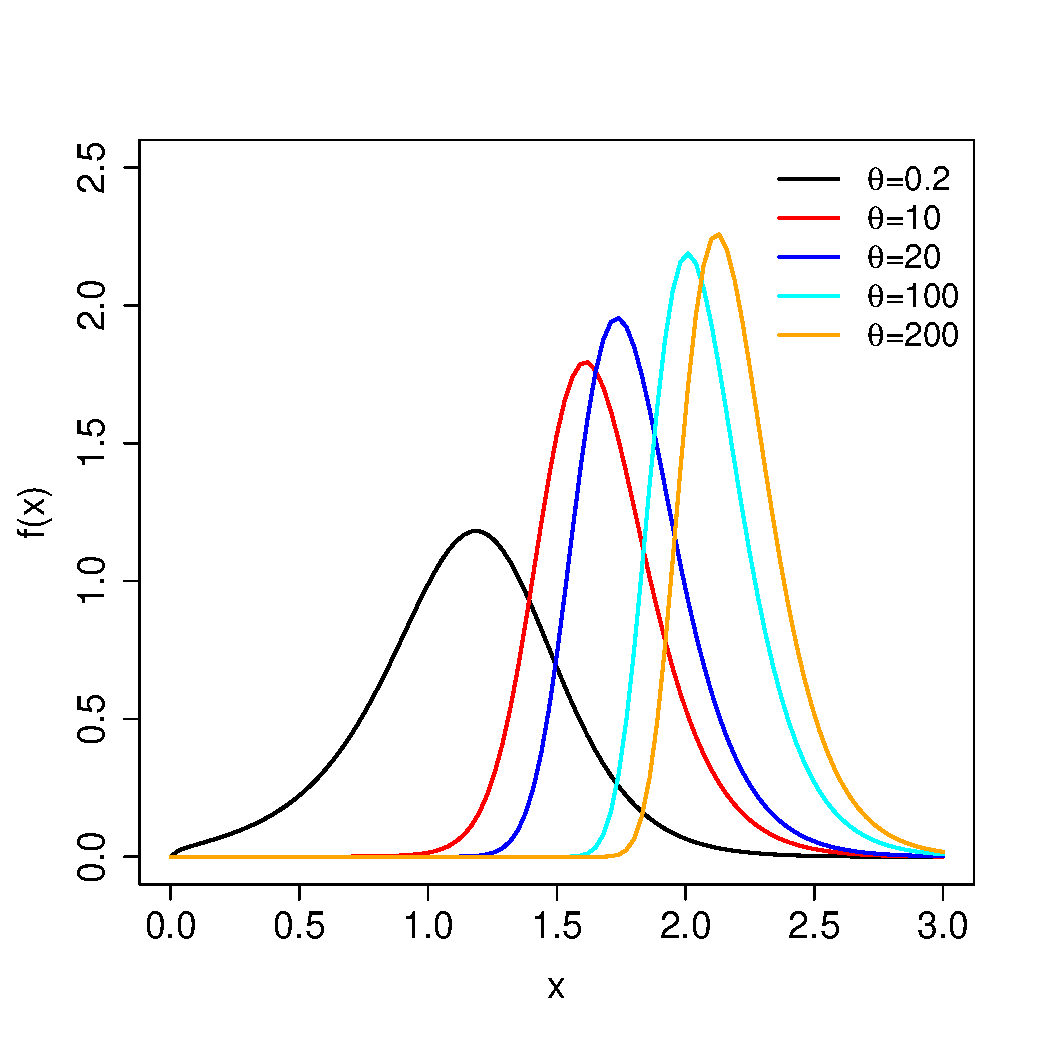
\includegraphics[width=3.5cm,height=5.5cm]{fdp_MOTPW_variando_theta.eps}~
		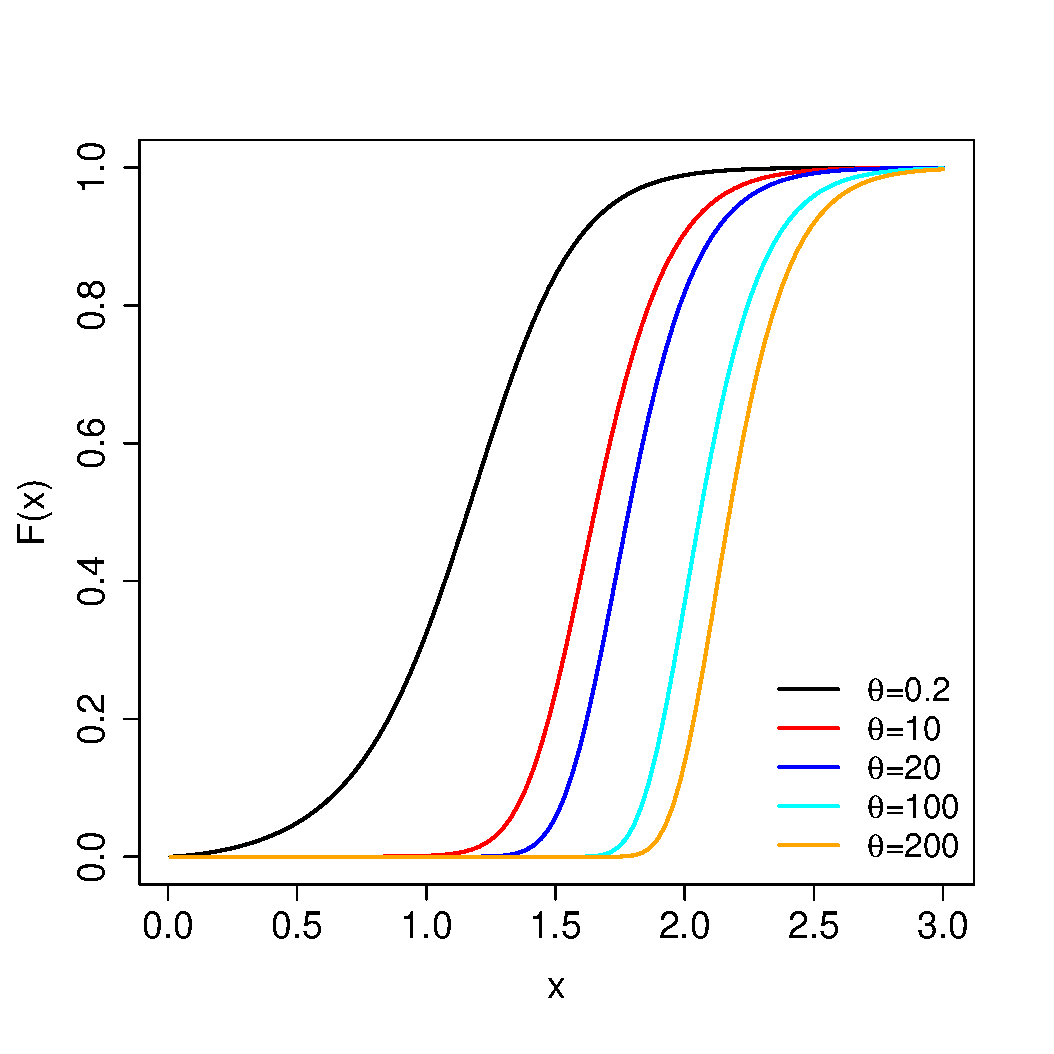
\includegraphics[width=3.5cm,height=5.5cm]{fda_MOTPW_variando_theta.eps}~
		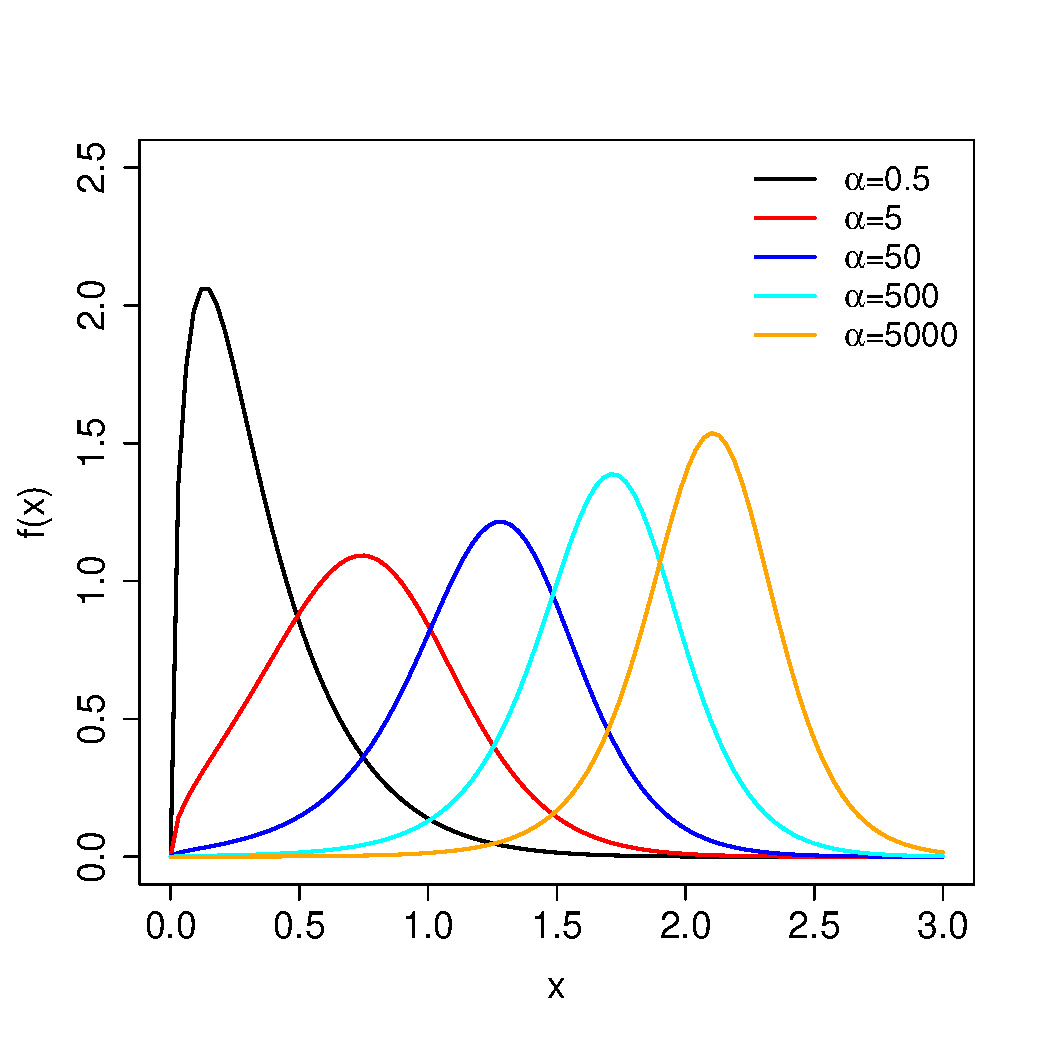
\includegraphics[width=3.5cm,height=5.5cm]{fdp_MOTPW_variando_alpha.eps}
		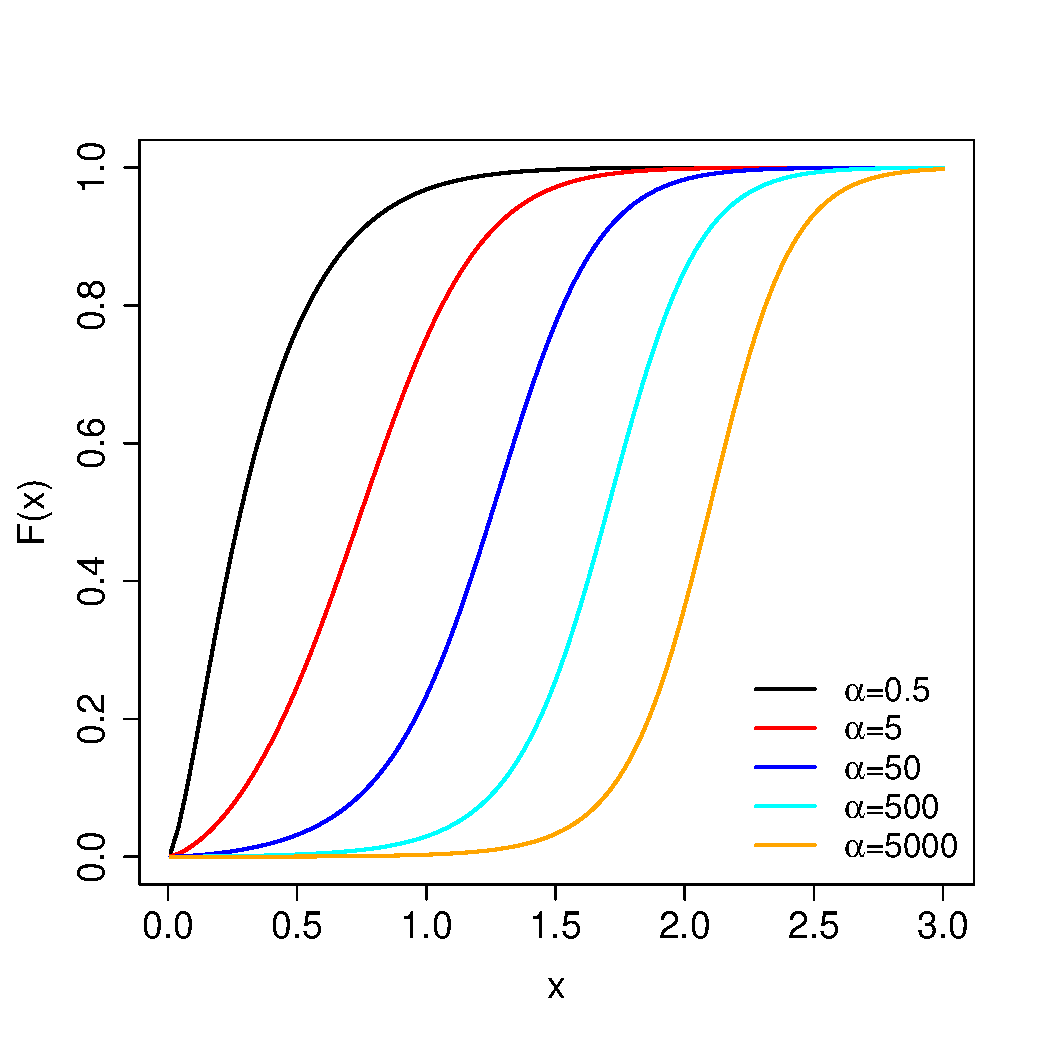
\includegraphics[width=3.5cm,height=5.5cm]{fda_MOTPW_variando_alpha.eps}
		\caption{Plots of the density and cumulative functions of the MOTPW distribution under four scenarios. (a) $\alpha=30$, $\lambda=2$, $\beta=1.5$, and varying $\theta$. (b)  $\alpha=30$, $\lambda=2$, $\beta=1.5$, and varying $\theta$. (c) $\theta=0.09$, $\lambda=2$, $\beta=1.5$, and varying $\alpha$. (d) $\theta=0.09$, $\lambda=2$, $\beta=1.5$,
			and varying  $\alpha$.}
		\label{fdp_e_fda_MOTPW}
	\end{center}
\end{figure}


\begin{figure}[!htb]\small
	\begin{center}
		(a)\hspace{3cm}(b)\hspace{3cm}(c)\hspace{3cm}(d)
		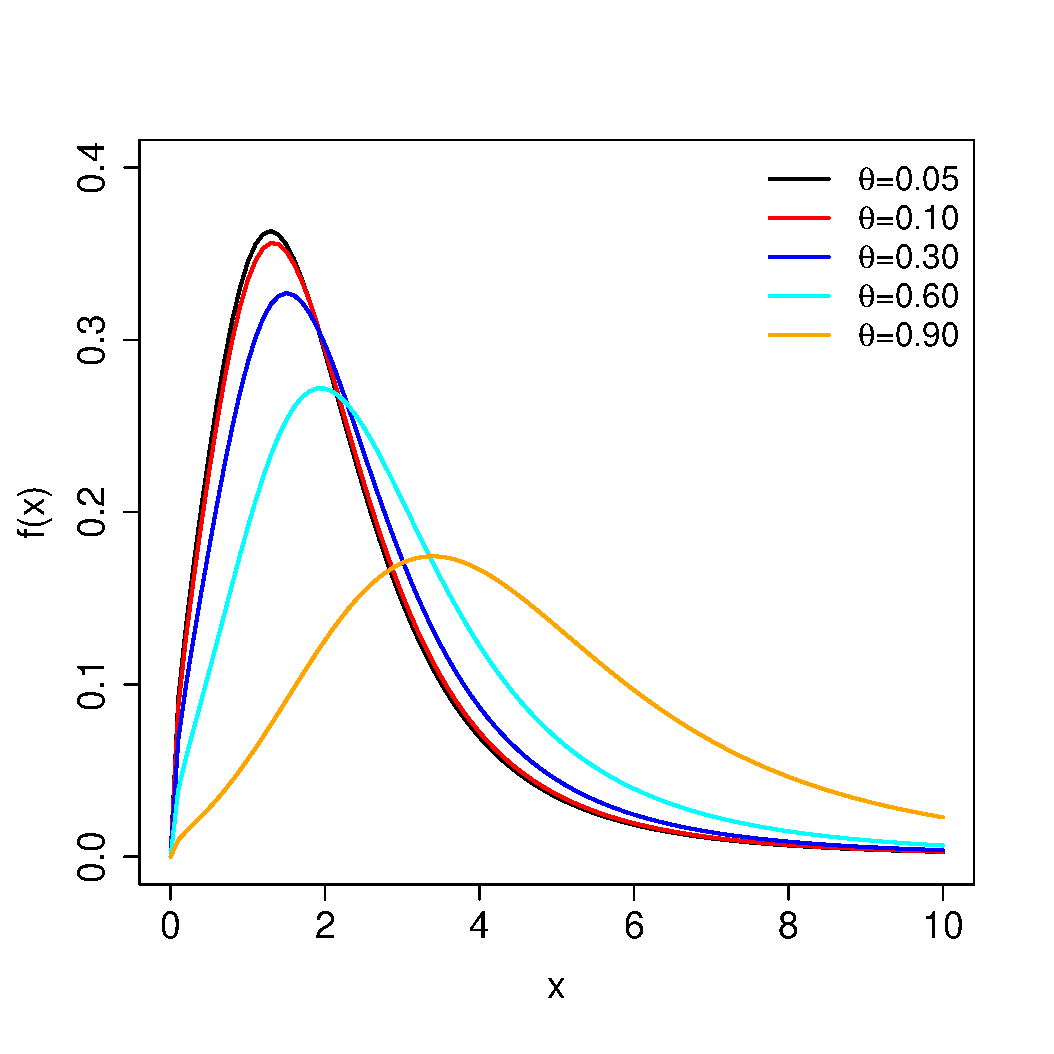
\includegraphics[width=3.5cm,height=5.5cm]{fdp_MOGBXII_variando_theta.eps}~
		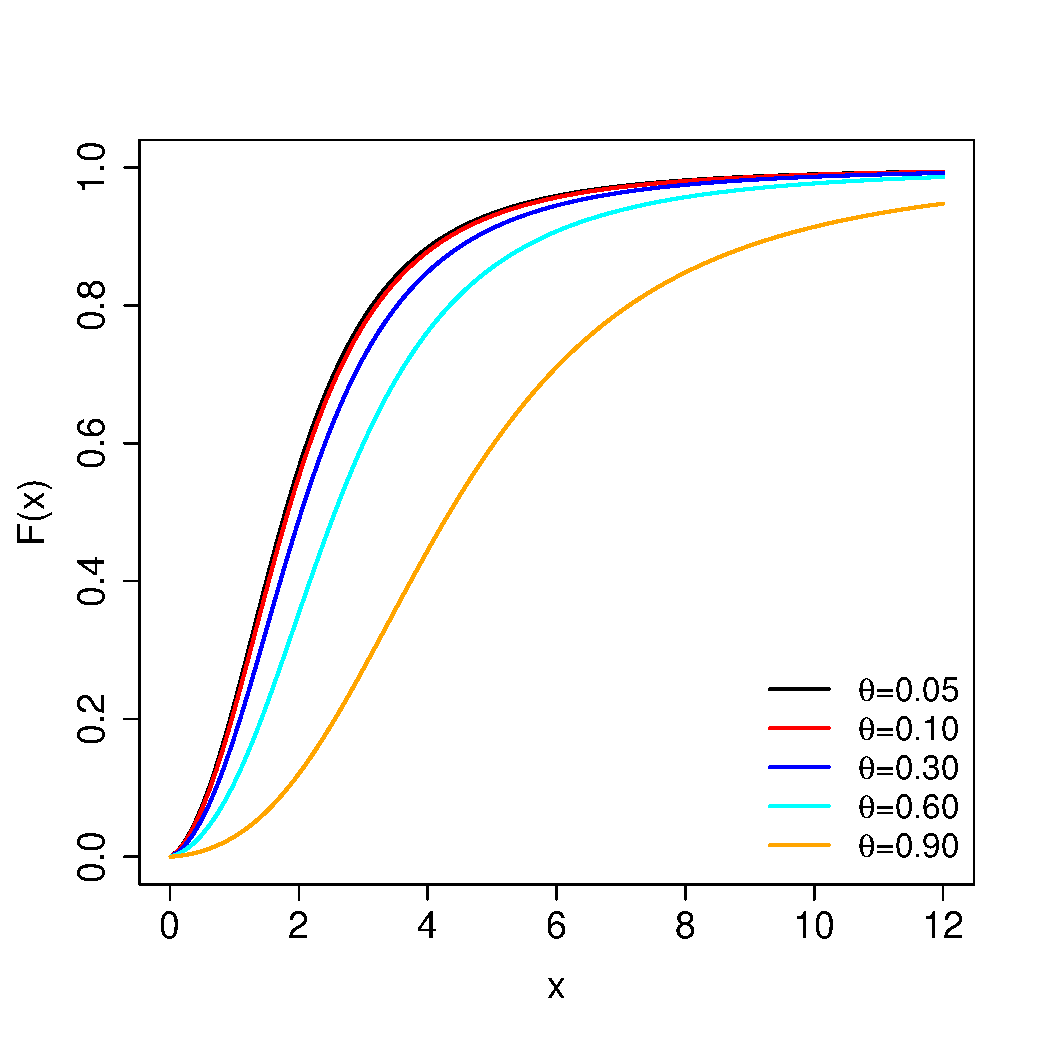
\includegraphics[width=3.5cm,height=5.5cm]{fda_MOGBXII_variando_theta.eps}~
		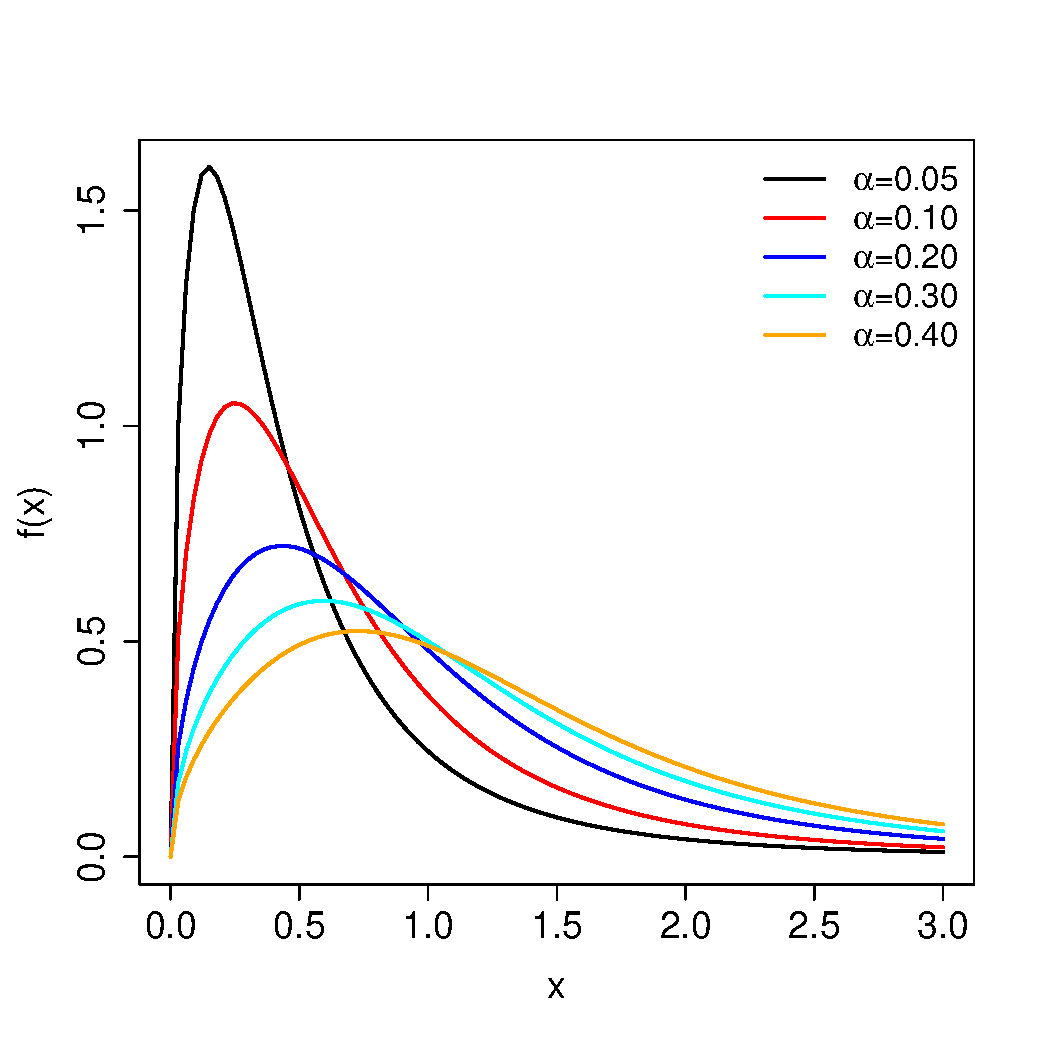
\includegraphics[width=3.5cm,height=5.5cm]{fdp_MOGBXII_variando_alpha.eps}
		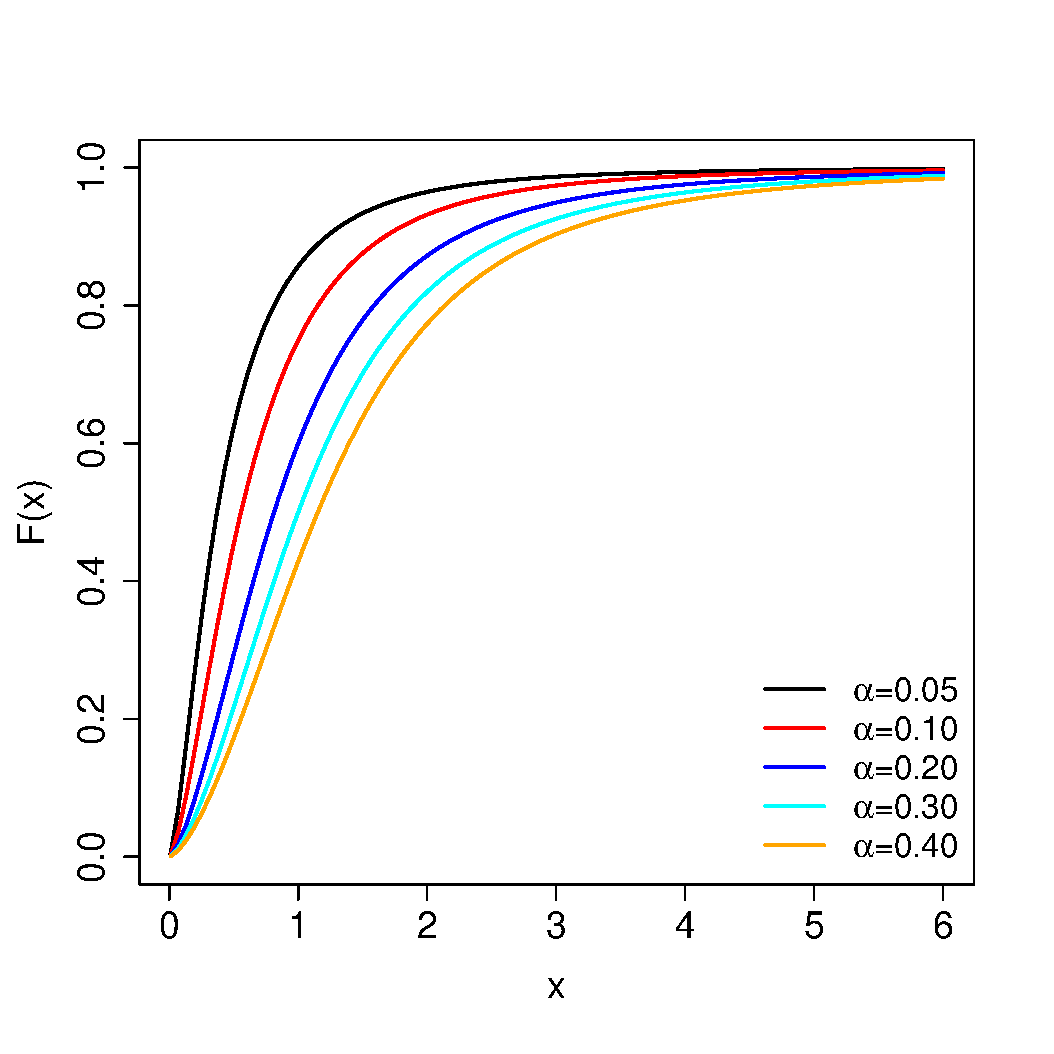
\includegraphics[width=3.5cm,height=5.5cm]{fda_MOGBXII_variando_alpha.eps}
\caption{Plots of the density and cumulative functions of the MOGBXII distribution under four scenarios. (a) $\alpha=10$, $\lambda=2$,
$\beta=1.5$, and varying $\theta$. (b) $\alpha=10$, $\lambda=2$, $\beta=1.5$, and varying $\theta$.  (c) $\theta=0.9$, $\lambda=2$, $\beta=1.5$, and varying  $\alpha$. (d)
$\theta=0.9$, $\lambda=2$, $\beta=1.5$, and varying  $\alpha$.}
		\label{fdp_e_fda_MOGBXII}
	\end{center}
\end{figure}


\begin{figure}[!htb]\small
	\begin{center}
		(a)\hspace{3cm}(b)\hspace{3cm}(c)\hspace{3cm}(d)\hspace{3cm}(e)	
		\includegraphics[width=3.5cm,height=5.5cm]{hrf_MOTPW_variando_theta_e_alpha.eps}~
		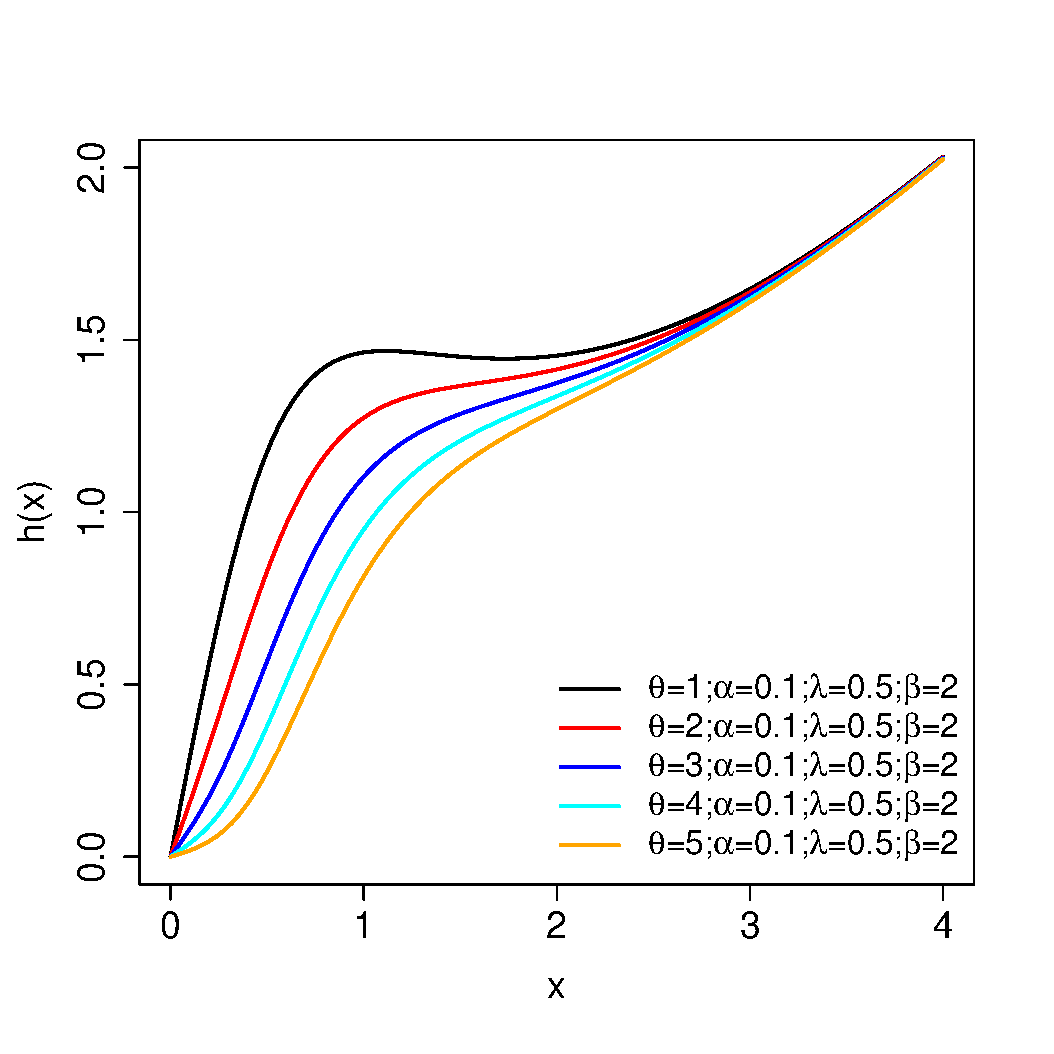
\includegraphics[width=3.5cm,height=5.5cm]{hrf_MOTPW_variando_theta.eps}~
		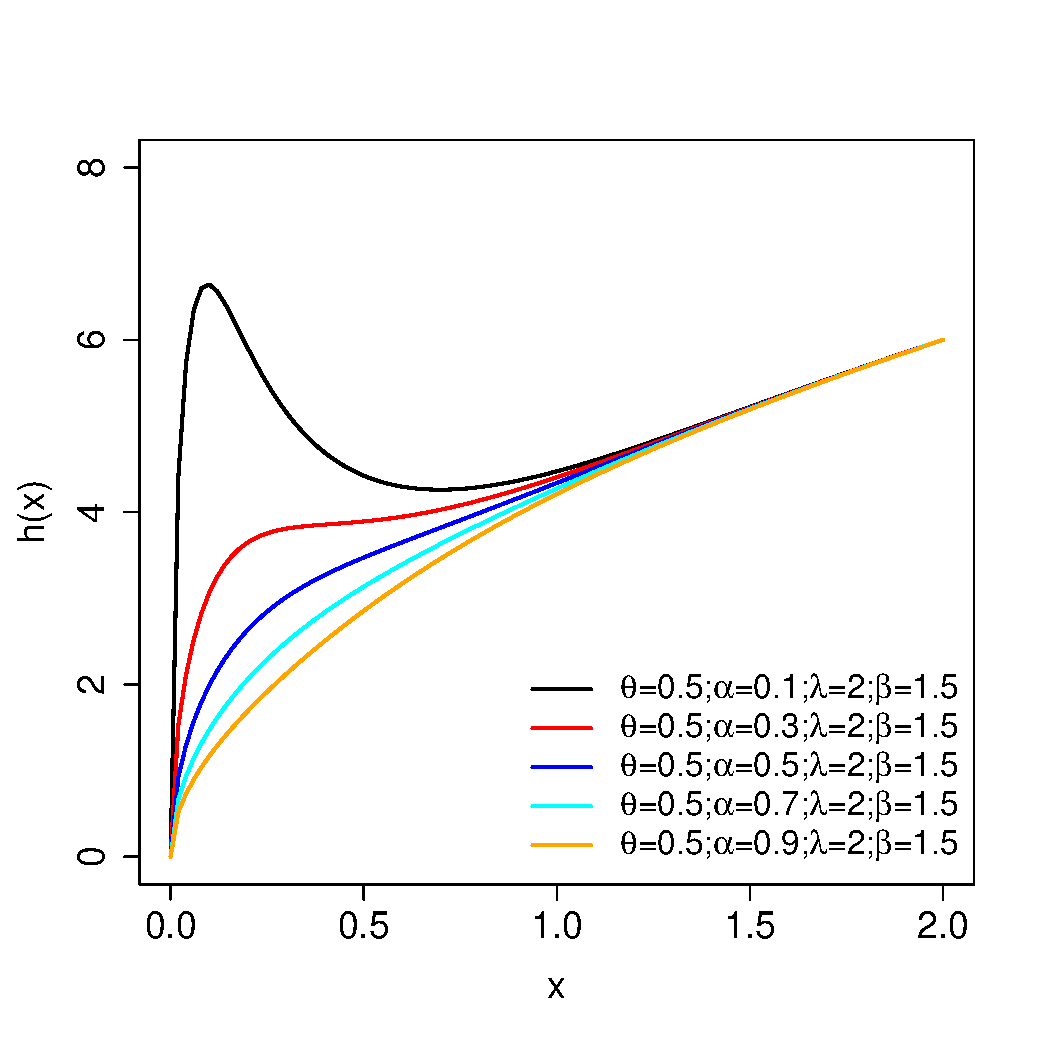
\includegraphics[width=3.5cm,height=5.5cm]{hrf_MOTPW_variando_alpha.eps}~
		\includegraphics[width=3.5cm,height=5.5cm]{hrf_MOTPW_variando_lambda.eps}~
		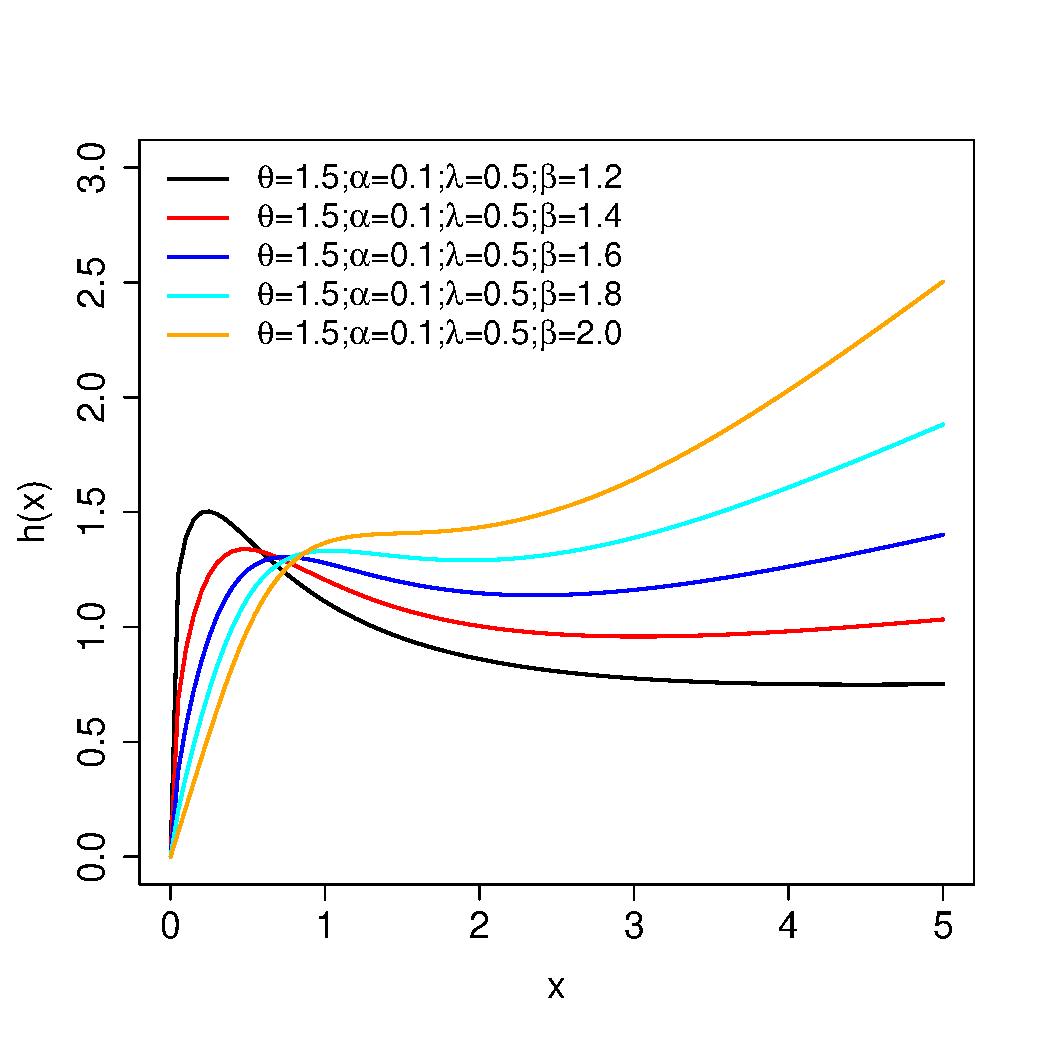
\includegraphics[width=3.5cm,height=5.5cm]{hrf_MOTPW_variando_beta.eps}
		\caption{\textcolor{red}{Plots of the hrf of the MOTPW model.}}
		\label{hrf}
	\end{center}
\end{figure}
	
{\color{red} We can note increasing, decreasing, and unimodal shapes for the hrf of the MOTPW distribution in Figure \ref{hrf}. 
Also, we see a slightly different hrf with increasing, decreasing and increasing shape.}



%\begin{figure}[!htb]\small
%	\begin{center}
%		(a)\hspace{3cm}(b)\hspace{3cm}(c)	
%		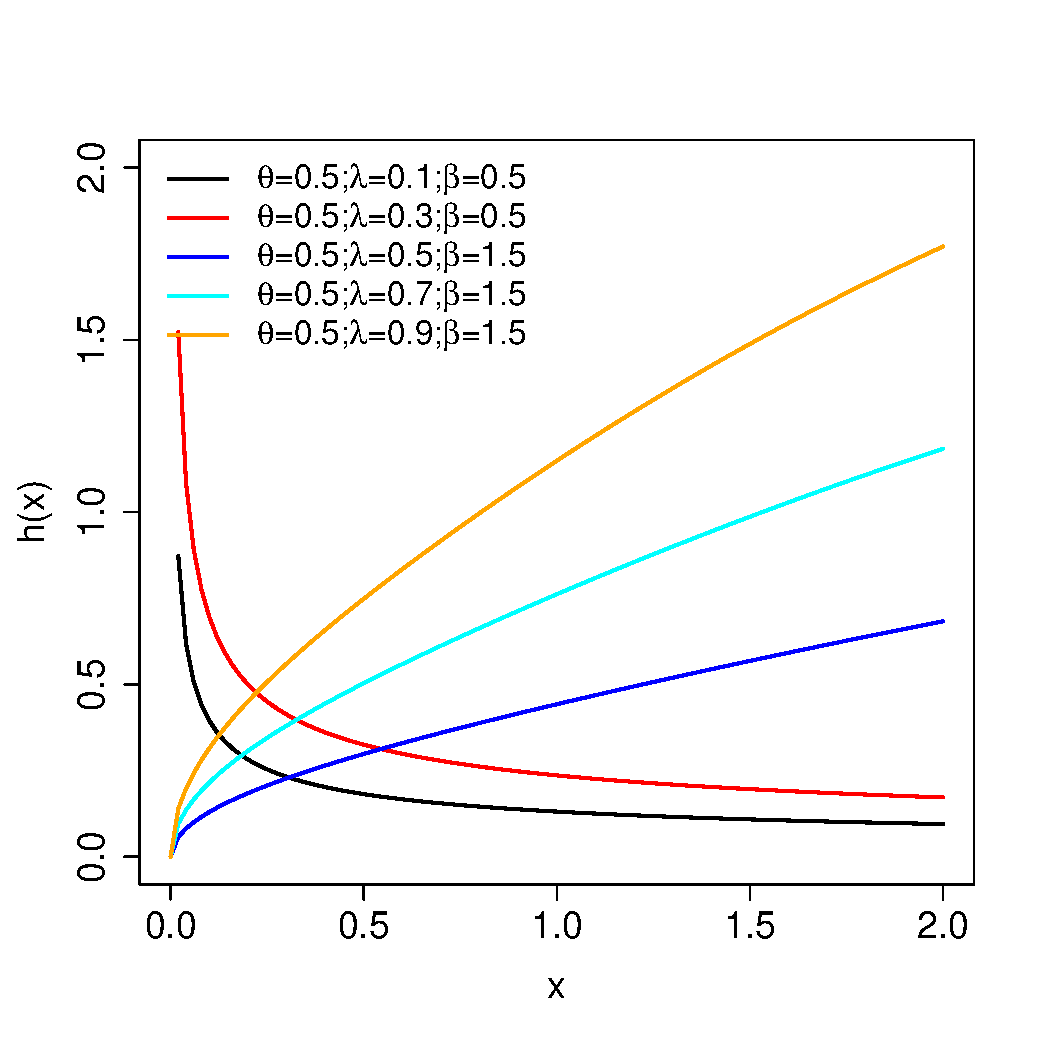
\includegraphics[width=3.5cm,height=5.5cm]{hrf_TPW_variando_lambda_e_beta.eps}~
%		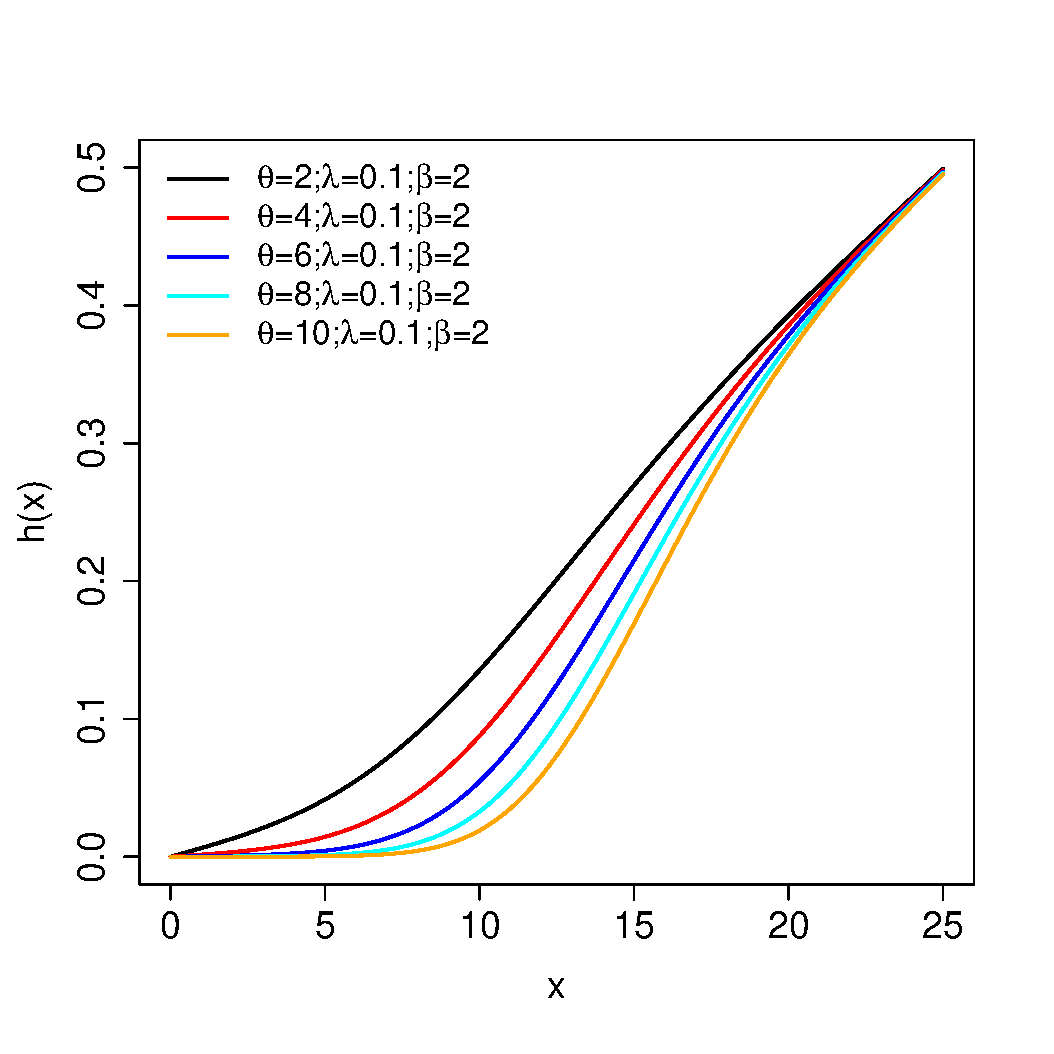
\includegraphics[width=3.5cm,height=5.5cm]{hrf_TPW_variando_theta.eps}~
%		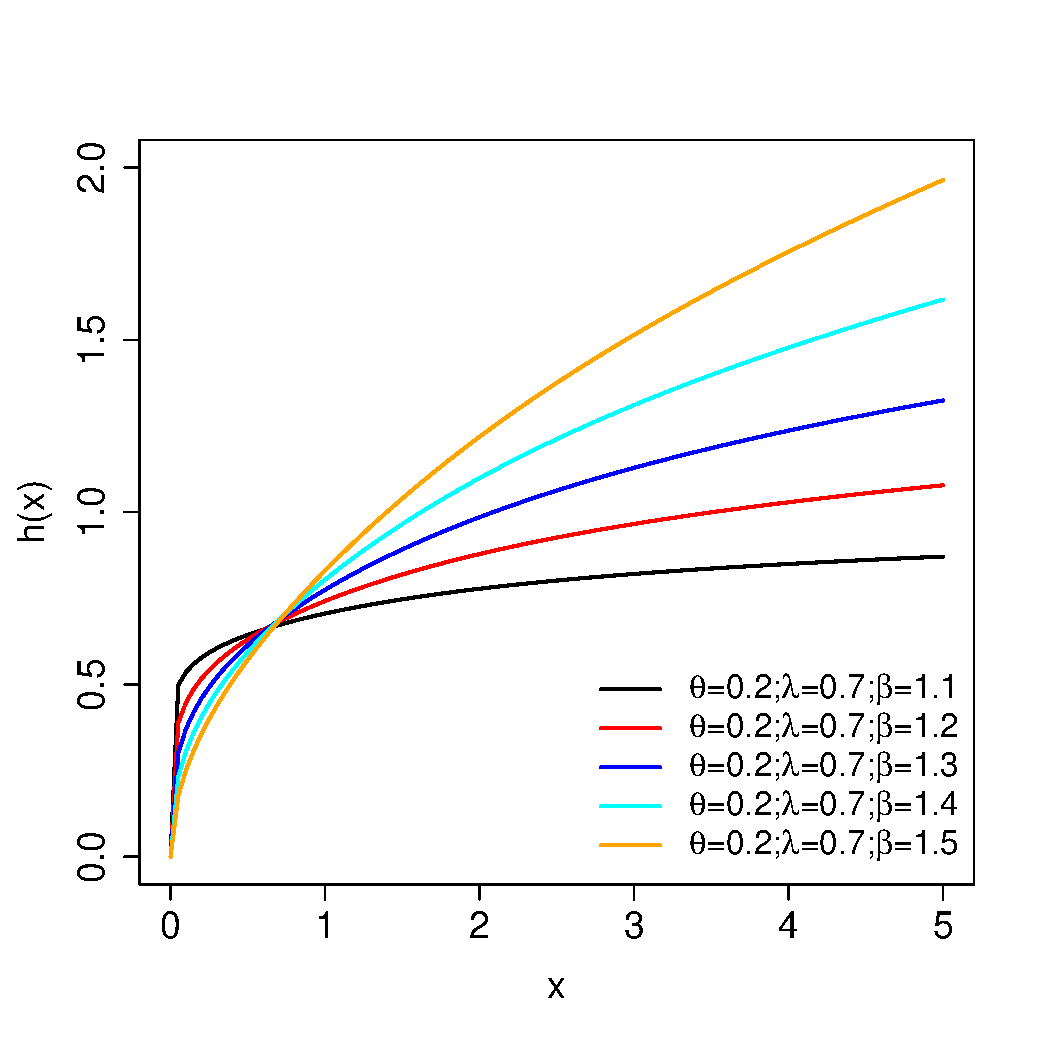
\includegraphics[width=3.5cm,height=5.5cm]{hrf_TPW_variando_beta.eps}
%		\caption{\textcolor{red}{Plots of the hrf TPW.}}
%		\label{hrf}
%	\end{center}
%\end{figure}
%	
	
Graphics comparing the histograms from two simulated data sets and the MOTPW and MOGBXII densities of $X$
under specified parameters are reported in Figure \ref{hist_MOTPW_MOGBXII}. They show good agreement between the simulated values
and these densities.
\begin{figure}[!htb]\small
	\begin{center}
		(a)\hspace{5cm}(b)\\					
		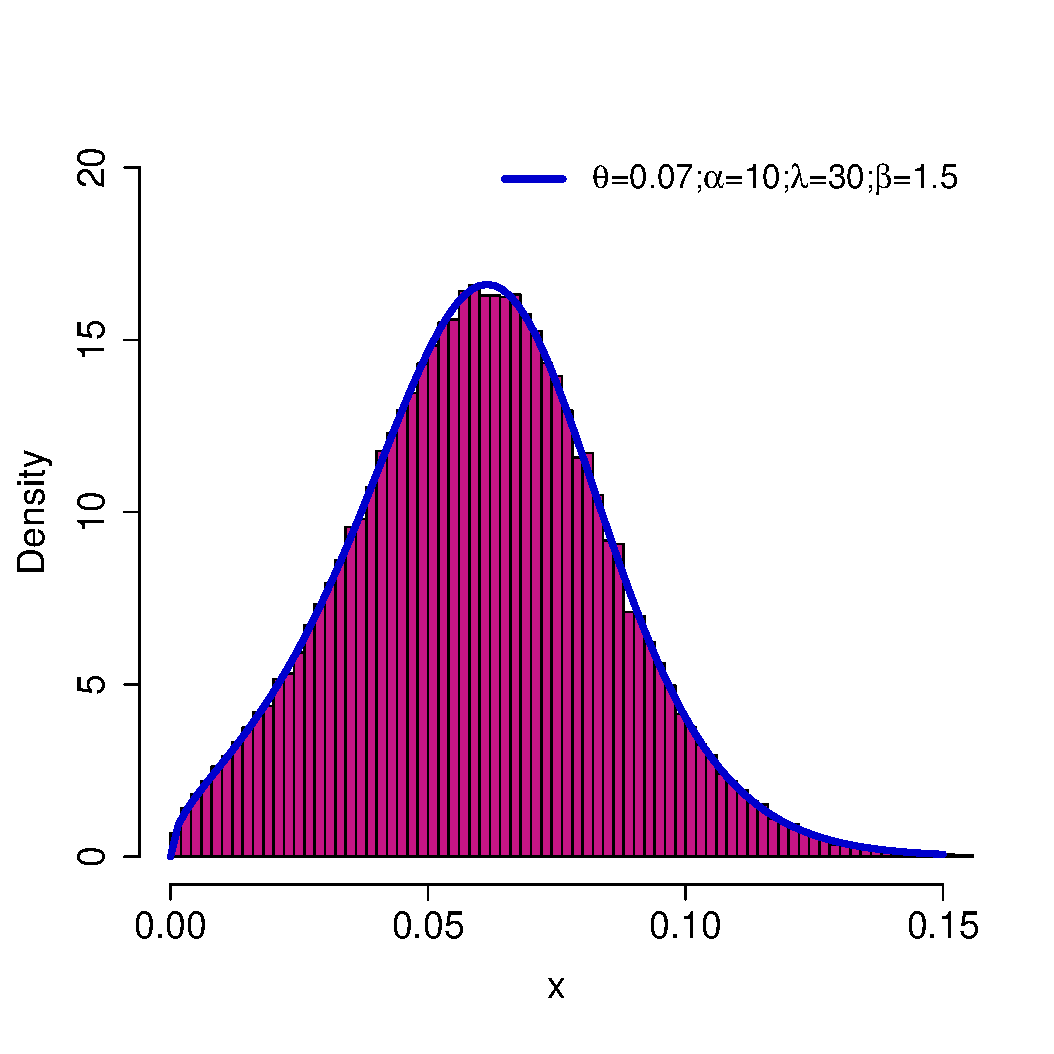
\includegraphics[width=5.5cm,height=5.5cm]{histograma_MOTPW.eps}~
		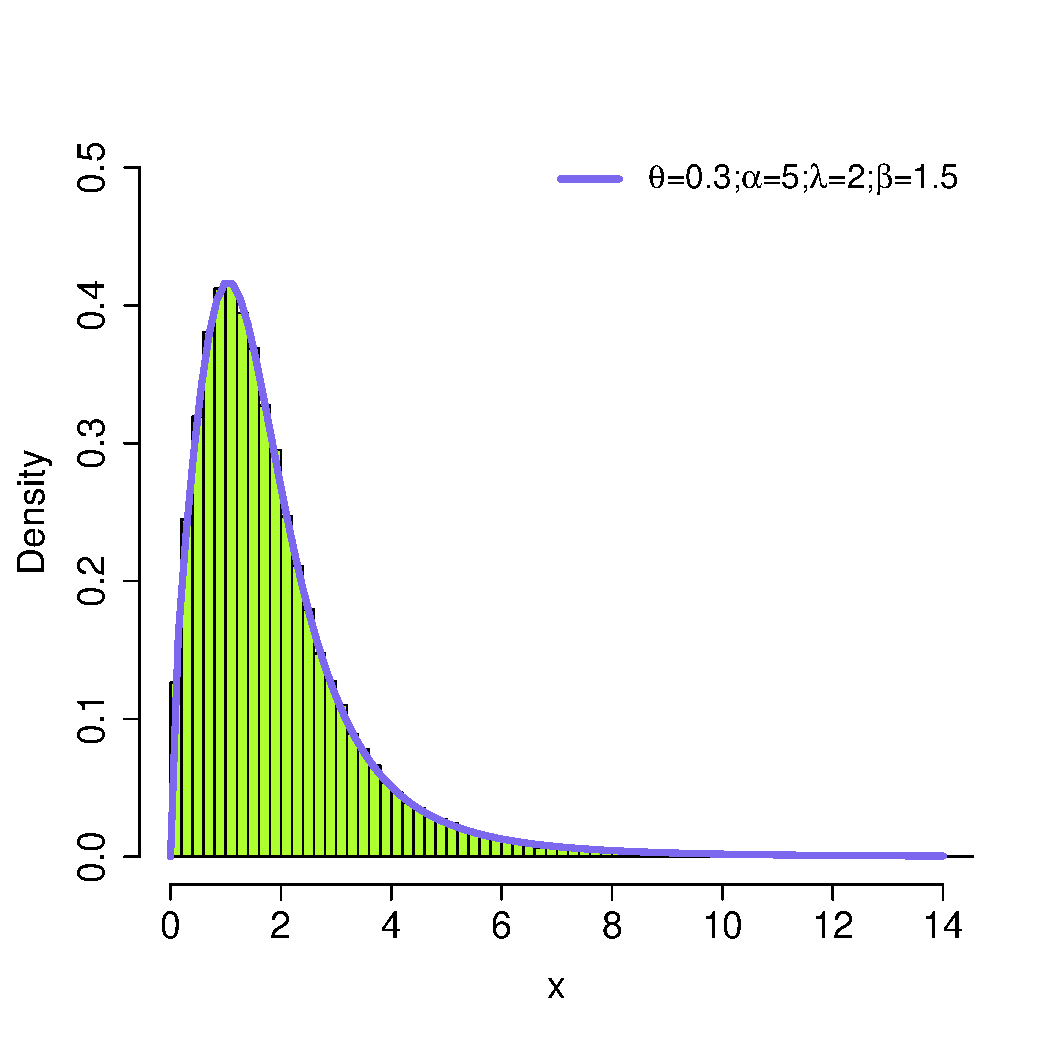
\includegraphics[width=5.5cm,height=5.5cm]{histograma_MOGBXII.eps}
		\caption{Plots of the MOTPW (a) and MOGBXII (b) densities and histograms of simulated data.}
		\label{hist_MOTPW_MOGBXII}
	\end{center}
\end{figure}




\section{Expansions}\label{expansions}

We obtain useful linear representations for the density functions of $X$ and $Y$ for two separated cases $\alpha\in(0,1)$
and $\alpha >1$. For $\alpha=1$, we have $H(z;1,\bm{\tau})=G(z;\bm{\tau})$.

By inserting (\ref{cdf_G}) in Equation (\ref{ucdfmax}) and letting $\bar{G}(x)=\bar{G}(x;\bm{\tau})$, we can write
\begin{eqnarray}\label{auxiliar}
F_X(x)=\sum_{n=1}^{\infty}\frac{p_n\,G(x)^n}{\left[1-\bar{\alpha}\bar{G}(x)\right]^n}.
\end{eqnarray}

First, we consider the density of the maximum $X$ when $\alpha\in(0,1)$. For $|z|<1$ and $n=1,2,\ldots$, the negative binomial expansion holds
\begin{equation}\label{taylor}
(1-z)^{-n}=\sum^{\infty}_{k=0}\, {-n \choose k}\,(-z)^k.
\end{equation}

Expanding $\left[1-\bar{\alpha}\bar{G}(z)\right]^{-n}$ as in Equation (\ref{taylor}) since $\alpha\in(0,1)$, we have
\begin{eqnarray*}
F_X(x)=\sum_{n=1}^{\infty}\sum^{\infty}_{k=0}\, {-n \choose k}\,(-\bar{\alpha})^k\,p_n\,\,G(x)^n\,[1-G(x)]^k.
\end{eqnarray*}

Henceforth, let $T_{s}\sim~$exp-G$(s)$ be the exponentiated-G (exp-G) random variable with power parameter $s>0$. Its 
cdf and pdf are $\Pi_s(x)=\Pi_s(x;\bm{\tau})=G(x;\bm{\tau})^s$ and $\pi_s(x)=\pi_s(x;\bm{\tau})=s\,G(x;\bm{\tau})^{s-1}\,g(x;\bm{\tau})$,
respectively. Many exp-G properties have been studied exhaustively by se\-veral authors \citep{Tahir2015}. We can write
\begin{eqnarray*}
F_X(x)=\sum_{n=1}^{\infty}\,w_{n,0}\,\Pi_n(x) +\sum_{n=1}^{\infty}\sum^{\infty}_{k=1}\,w_{n,k}\,\Pi_n(x)\,[1-G(x)]^k,
\end{eqnarray*}
where $w_{n,k}=w_{n,k}(\alpha,\theta)={-n \choose k}\,(-\bar{\alpha})^k\,p_n$ for $n=1,2,\ldots$ and $k=0,1,\ldots$
Further, using the binomial theorem, we obtain
\begin{eqnarray*}
F_X(x)=\sum_{n=1}^{\infty}\,w_{n,0}\,\Pi_n(x) +\sum_{n=1}^{\infty}\sum^{\infty}_{k=1}\sum^{k}_{i=0}\,w_{n,k,i}\,\Pi_{n+i}(x),
\end{eqnarray*}
where $w_{n,k,i}=(-1)^i\,{k \choose i}\,w_{n,k}$ for $i=0,1,\ldots,k$.

By differentiating the last equation, we obtain
\begin{eqnarray}\label{densityX}
f_X(x)=\sum_{n=1}^{\infty}\,w_{n,0}\,\pi_n(x) +\sum_{n=1}^{\infty}\sum^{\infty}_{k=1}\sum^{k}_{i=0}\,w_{n,k,i}\,\pi_{n+i}(x).
\end{eqnarray}

We now move to the density of the maximum $X$ when $\alpha>1$. We modify the denominator in (\ref{auxiliar})
\begin{eqnarray*}
F_X(x)=\sum_{n=1}^{\infty}\frac{p_n\,G(x)^n}{\alpha^n \,\left[1-(1-\alpha^{-1})G(x)\right]^n}
\end{eqnarray*}
and then apply Equation (\ref{taylor}) to find
\begin{eqnarray*}
F_X(x)=\sum_{n=1}^{\infty}\sum^{\infty}_{k=0}\,v_{n,k}\,\Pi_{n+k}(x),
\end{eqnarray*}
where $v_{n,k}=v_{n,k}(\alpha,\theta)=(-1)^k\,{-n \choose k}\,\alpha^{-n}\,(1-\alpha^{-1})^k\,p_n$ (for $n=1,2,\ldots$ and $k=0,1,\ldots$).
By differentiating $F_X(x)$, the density of $X$ follows as
\begin{eqnarray}\label{densityX1}
f_X(x)=\sum_{n=1}^{\infty}\sum^{\infty}_{k=0}\,v_{n,k}\,\pi_{n+k}(x).
\end{eqnarray}


Next, we consider the density of the minimum $Y$. By inserting (\ref{survivor_G}) in Equation (\ref{ucdfmin}), we have
\begin{eqnarray}\label{auxiliar1}
F_Y(y)=1-\sum_{n=1}^{\infty}\frac{\alpha^n\,p_n\,\bar{G}(y)^n}{\left[1-\bar{\alpha}\bar{G}(y)\right]^n}.
\end{eqnarray}

For $\alpha\in(0,1)$, we apply expansion (\ref{taylor}) in the last equation to
\begin{eqnarray*}
F_Y(y)=1-\sum_{n=1}^{\infty}\sum^{\infty}_{k=0}q_{n,k}\,\bar{G}(y)^{n+k},
\end{eqnarray*}
where $q_{n,k}=q_{n,k}(\alpha,\theta)=(-1)^k\,{-n \choose k}\,\bar{\alpha}^k\,\alpha^n\,p_n$
for $n=1,2,\ldots$ and $k=0,1,\ldots$

By using the binomial theorem in $\bar{G}(y)^{n+k}$, we have
\begin{eqnarray*}
F_Y(y)=1+\sum_{n=1}^{\infty}\sum^{\infty}_{k=0}\sum^{n+k}_{i=0}\,q_{n,k,i} \,\Pi_i(y),
\end{eqnarray*}
where $q_{n,k,i}=(-1)^{i+1}\,{n+k \choose i}\,q_{n,k}$ for $i=0,1,\ldots,n+k$.

By differentiating $F_Y(y)$, the density of $Y$ can be expressed as
\begin{eqnarray}\label{densityY}
f_Y(y)=\sum_{n=1}^{\infty}\sum^{\infty}_{k=0}\sum^{n+k}_{i=1}\,q_{n,k,i}\,\pi_i(y).
\end{eqnarray}


Finally, we obtain the density of $Y$ when $\alpha> 1$. By changing the
denominator in Equation (\ref{auxiliar1}), we have
\begin{eqnarray*}
F_Y(y)=1-\sum_{n=1}^{\infty}\frac{p_n\,\bar{G}(y)^n}{\left[1-(1-\alpha^{-1})G(y)\right]^n}.
\end{eqnarray*}

Applying expansion (\ref{taylor}) in the last equation
\begin{eqnarray*}
F_Y(y)=1-\sum_{n=1}^{\infty}\sum^{\infty}_{k=0}t_{n,k}\,\bar{G}(y)^n\,G(y)^k ,
\end{eqnarray*}
where $t_{n,k}=t_{n,k}(\alpha,\theta)=(-1)^k\,(1-\alpha^{-1})^k\,{-n \choose k}\,p_n$ (for $n=1,2,\ldots$ and $k=0,1,\ldots$).

Using the binomial theorem, we can rewrite $F_Y(y)$ as
\begin{eqnarray*}
F_Y(y)=1+\sum_{n=1}^{\infty}\sum^{\infty}_{k=0}\sum^{n}_{i=0}\,t_{n,k,i}\,\Pi_{i+k}(y),
\end{eqnarray*}
where $t_{n,k,i}=(-1)^{i+1}\,{n \choose i}\,t_{n,k}$ for $i=0,1,\ldots$ By simple differentiation
\begin{eqnarray}\label{densityY1}
f_Y(y)=\sum_{n=1}^{\infty}\sum^{\infty}_{k=0}\sum^{n}_{i=0}\,t_{n,k,i}\,\pi_{i+k\ge 1}(y),
\end{eqnarray}
where $\pi_{i+k\ge 1}(y)$ is the exp-G density with power parameter $i+k \ge 1$.

Equations (\ref{densityX}), (\ref{densityX1}), (\ref{densityY}) and (\ref{densityY1}) are the main results of this section.
These linear representations have great utility for deriving structural properties of the maximum $X$ and minimum $Y$ from well-known
exp-G properties. More than thirty five exp-G models have been studied
so far and then it is possible to construct at least three hundred fifty ($70 \times 5$) MOPS-G models with properties
determined from those exp-G properties. We can use statistical platforms with ten terms to have precise results.

\section{Numerical evaluation}

In order to evaluate the mathematical results presented in the previous sections, a package was implemented using the programming language R, \cite{rlang}. The \textbf{MarshallOlkinPSG} package was implemented in a generic way, that is, its most important functions allow generalizations, being possible to inform any baseline $G$ distribution or even inform a zero-truncated power series (PS) distribution. 

The library code can be obtained from GitHub, at \href{GitHub}{https://github.com/prdm0/MarshallOlkinPSG}. On the library's website (see \href{website}{https://prdm0.github.io/MarshallOlkinPSG}) it is possible to obtain more information on the functions implemented through the documentation and usage examples.

To install the package hosted and maintained on GitHub, it is necessary to previously install the \textbf{remotes} library. With the prerequisite met, the package \textbf{MarshallOlkinPSG} can be installed by doing:

\begin{lstlisting}
# Install the remotes package: 
# install.packages("remotes")
remotes::install_github("prdm0/MarshallOlkinPSG", force = TRUE)
\end{lstlisting}

The function \texttt{eq\_19()} of the package implements Eq. \ref{densityX1} and can be compared, for example, with the MOTPW distribution presented in Eq. \ref{MOTPW1}. To facilitate comparison, the function \texttt{pdf\_theorical ()} implements the MOTPW1 density function. By doing \texttt{help(eq\_19)} it is possible to have access to an example of comparison of the two equations, where it is noted that Eq. \ref{densityX1} approximates Eq. \ref{MOTPW1} very well, when finite sums are considered in the case of applied problems. In other words, it is observed that in the same configurations, the results achieved by the function \texttt{eq\_19()} approximates very well those achieved using \texttt{pdf\_theorical()}.

The function \texttt{eq\_19()} will also allow any baseline to be informed, just passing the cumulative distribution function $G$ as an argument of \texttt{eq\_19()}.

Using the function \texttt{eval\_plot\_moptw()}, it is possible to observe and numerically validate, more clearly, the Eq. \ref{densityX1} by means of graphical observation. In addition, it is noted that few sums are needed to obtain a reasonable level of precision, as can be seen in Figure \ref{fig:numerical}, where six or eight terms provide very reasonable approximations.

\begin{figure}[H]\label{fig:numerical}
\centering
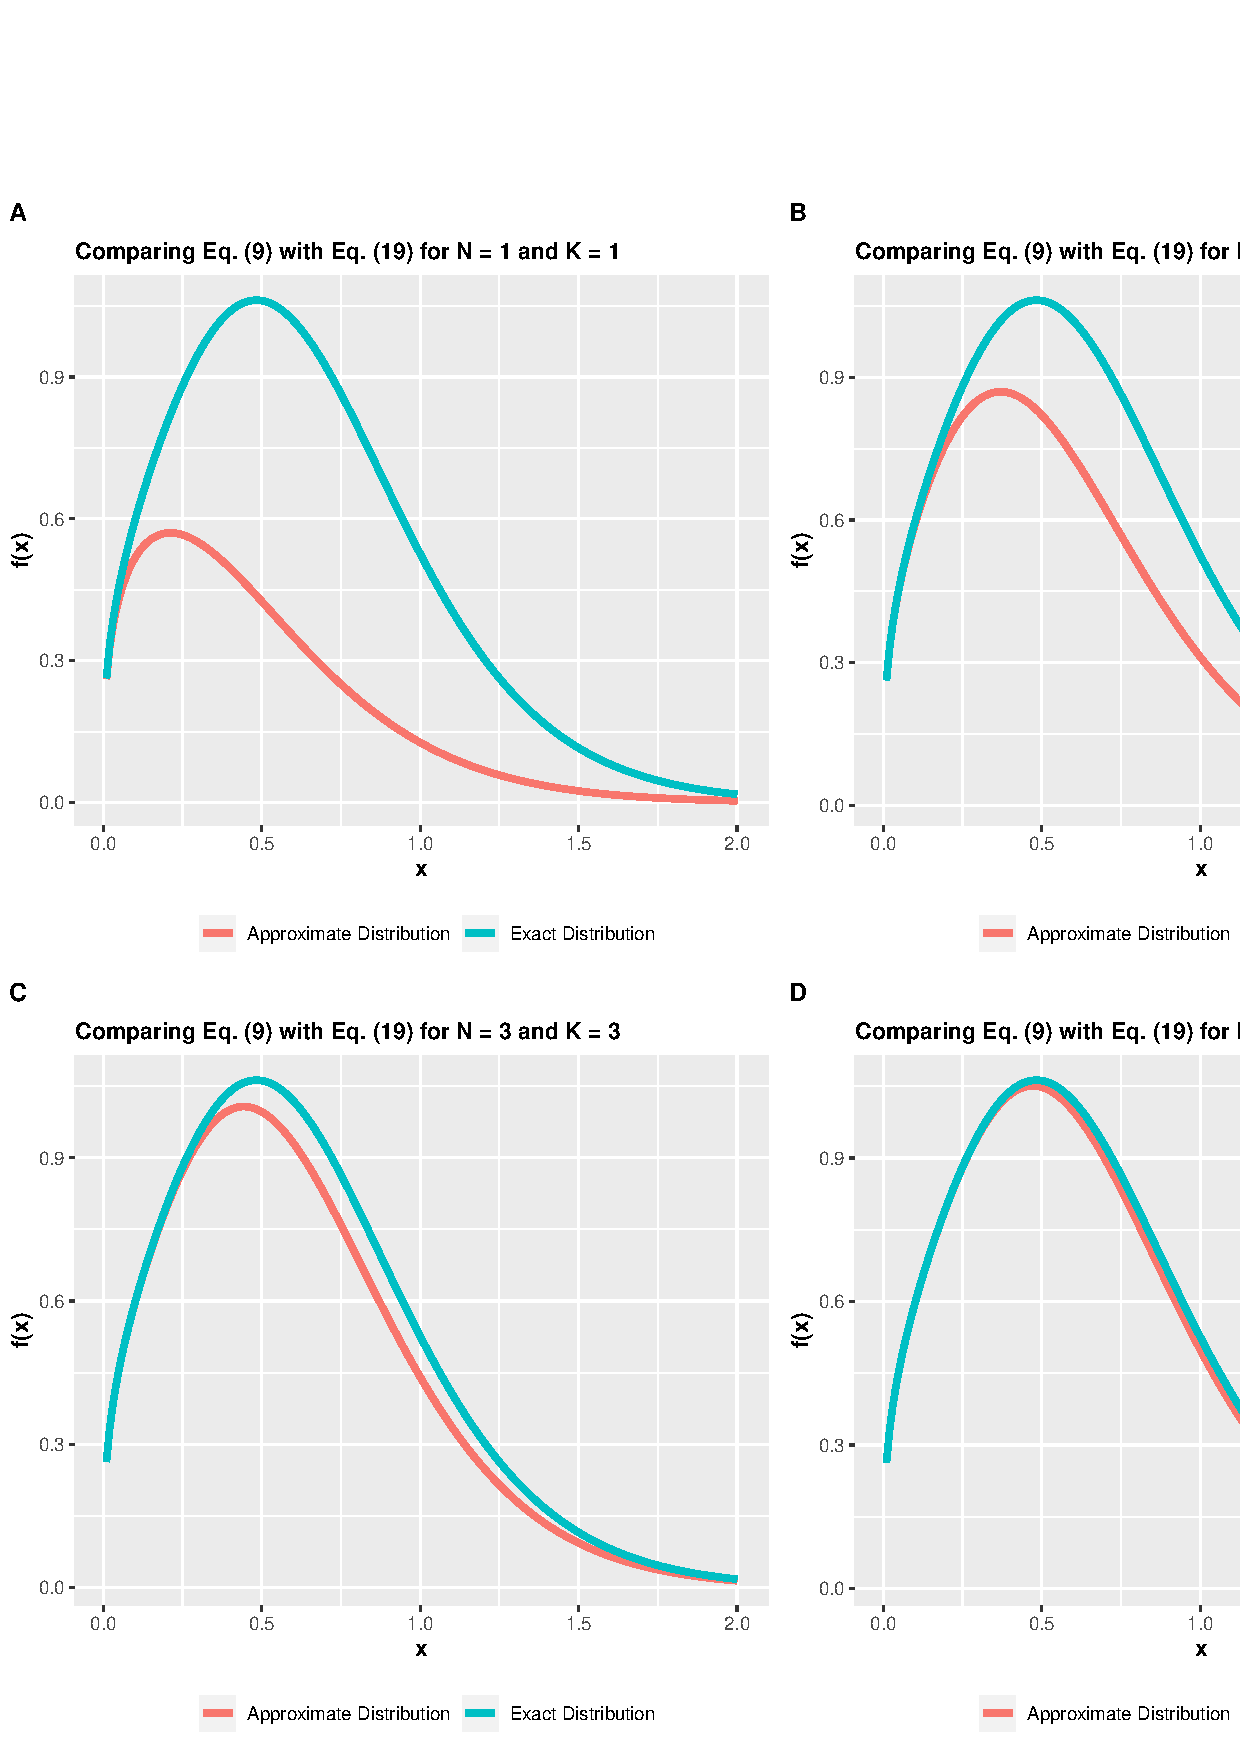
\includegraphics[scale = 0.7]{numerical_evaluation.png}
\caption{Numerical evaluation of Eq. \ref{densityX1} when considering finite sums, with $N$ and $K$ being the total number of terms considered in the exterior and interior sum, respectively, for $\alpha = 1.2$, $\theta = 1.5$, $\beta = 1.33$ and $\lambda = 2$.}
\end{figure}

\section{Properties}\label{gen_proper}


We now provide some mathematical properties of $T_s$ that can be easily utilized in the linear representations of the previous
section to find the corresponding properties of $X$ and $Y$.

The $n$th ordinary moment of $T_s$ has the form
\begin{equation}\label{moments}
\mu_n^{\prime}=E(T_s^n)=s\,\int_{-\infty}^{\infty} t^n\,G(t;\bm{\tau})^{s-1}\,g(t;\bm{\tau}) dt=s\,\int_{0}^{1} Q_G(u)^n\,u^{s-1} du,
\end{equation}
where $Q_G(u;\bm{\tau})=G^{-1}(u;\bm{\tau})$ is the qf of $G$.

Explicit expressions for several exp-G moments can be determined from (\ref{moments}).

The $n$th incomplete moment of $T_s$ follows the previous algebra
\begin{eqnarray}\label{incomplete}
m_{n}(y) = E(T_s^n|T_s<y)=s\,\int_{0}^{G(y;\bm{\tau})} Q_G(u)^n u^{s-1} du,
\end{eqnarray}
where the integral can be calculated for the great majority of G distributions. The first incomplete moment $m_{1}(y)$ is the
most important case of (\ref{incomplete}) to find mean deviations and Lorenz and Bonferroni curves.

The moment generating function (mgf) of $T_s$ follows as
\begin{equation}\label{mgf}
M(w)=E(\rm{e}^{w T_s})=s\,\int_{-\infty}^{\infty} \rm{e}^{w t}\,G(t;\bm{\tau})^{s-1}\,g(t;\bm{\tau}) dt=s\,\int_{0}^{1} \exp\left[w\, Q_G(u)\right]\,u^{s-1} du.
\end{equation}

The mgfs of exp-G distributions con be determined from Equation (\ref{mgf}).



\section{Estimation}\label{sec:estimation}

Th MLEs are appropriate at least in large samples to determine confidence intervals for the parameters.
We consider the random variable $X$ defined from Equations (\ref{pdfmo}) and (\ref{ucdfmax}) for
any baseline G with any unknown parameter vector $\psin =(\alpha,\theta,\bm{\tau})^{T}$.
By simple differentiation of (\ref{ucdfmax}), the density of $X$ takes the form
\begin{eqnarray}\label{maxdensity}
f_X(x;\alpha,\theta,\bm{\tau})=\frac{\alpha\,\theta\,g(x;\bm{\tau})\,C^{\prime}\left(\theta\,H(x;\alpha,\bm{\tau})\right)}{C(\theta)\,[1-\bar{\alpha}\bar{G}(x;\bm{\tau})]^2},
\end{eqnarray}
where $C^{\prime}(\cdot)$ follows from (\ref{eq1}) and
$H(x;\alpha,\bm{\tau})=G(x;\bm{\tau})/\left[1-\bar{\alpha}\,\bar{G}(x;\bm{\tau})\right]$.

The log-likelihood function for $\psin$ from a random sample \textcolor{red}{$x_{1},\ldots,x_{n}$} of $X$ is
\begin{eqnarray}
\ell &=&\ell (\psin)=\log\left[\frac{\alpha\,\theta}{C(\theta)}\right]+\sum_{i=1}^n
\log\left[g(x_i;\bm{\tau})\right]+\sum_{i=1}^n
\log\left[C^{\prime}\left(\theta\,H(x_i;\alpha,\bm{\tau})\right)\right]\nonumber\\
&-&2\,\sum_{i=1}^n
\log\left[1-\bar{\alpha}\bar{G}(x;\bm{\tau})\right].\label{log1}
\end{eqnarray}

A similar development can be conducted for the random variable $Y$ defined from Equation (\ref{ucdfmin}) for any baseline G.

We can find the MLE $\widehat{\psin}$ by maximizing Equation (\ref{log1}) using the \texttt{MaxBFGS} sub-routine (\texttt{Ox} program), 
\texttt{optim} function (\texttt{R}), and \texttt{PROC NLMIXED} (\texttt{SAS}). 
The {\it AdequacyModel} package can also maximize (\ref{log1}) using the PSO (particle swarm optimization)
approach from the quasi-Newton BFGS, Nelder-Mead and simulated-annealing methods to maximize the log-likelihood function and it does not require
initial values. Details are available at {\tt https://rdrr.io/cran/AdequacyModel/}.

\textcolor{red}{These scripts can be executed for a wide range of initial values and may lead to more
than one maximum. However, in these cases, we consider the MLEs corresponding to the largest value of the maximum log-likelihood.
There are sufficient conditions for the existence of these estimates such as compactness of the parameter space and the concavity of the log-likelihood function, but they can exist even when the conditions are not satisfied. In general, there is no explicit solution for the estimates from maximizing (\ref{log1}),
but we can establish theo\-re\-tical conditions on their existence and uniqueness for very special models by examining the ranges of the
score components.}




\section{Regression}\label{sec:regression}

Consider that  \textcolor{red}{$X_1,\ldots,X_n$ are independent random variables from any distribution in (\ref{MOTPW1}) assuming
that the parameters $\lambda$ and $\lambda$ vary through them}. We propose a new regression based on the response variable in (\ref{MOTPW1})
with the systematic components
\begin{eqnarray}\label{reg}
\lambda_{i}=\exp(\vn_{i}^{T}\etn_1)\quad \quad \mbox{and}\quad\quad
\beta_{i}=\exp(\vn_{i}^{T}\etn_2), \quad i=1,\ldots,n,
\end{eqnarray}
respectively, where \textcolor{red}{$\vn_{i}^{T}=(v_{i1},\ldots,v_{ip})$},
\textcolor{red}{$\etn_1=(\eta_{11},\ldots,\eta_{1p})^{T}$} and \textcolor{red}{$\etn_2=(\eta_{21},\ldots,\eta_{2p})^{T}$}.
Equations (\ref{MOTPW1}) and (\ref{reg}) define the MOTPW regression.
For $\alpha=1$, it follows the {\it truncated Poisson Weibull} (TPW) regression.

In a similar manner, we can construct many other regressions based on other MOPS-G distributions defined
from Equations (\ref{ucdfmax}) and (\ref{ucdfmin}).

The log-likelihood function for the vector $\psin=(\alpha,\theta,\etn_{1}^{T},\etn_{2}^{T})^{T}$
from the MOTPW regression can be reduced to
\begin{eqnarray}\label{veroy}
l(\psin)&=&n\log\left[\frac{\alpha\,\theta}{\exp(\theta)-1}\right]+\sum_{i=1}^{n}\log(\beta_{i})+\sum_{i=1}^{n}\beta_{i}\log(\lambda_{i})
+\sum_{i=1}^{n}(\beta_{i}-1)\log(x_{i})-\nonumber \\&&
\sum_{i=1}^{n}(\lambda_{i}x_{i})^{\beta_{i}}-\sum_{i=1}^{n}\log\left\{1-\bar{\alpha}\exp[-(\lambda_{i}x_{i})^{\beta_{i}}]\right\}
+\theta\sum_{i=1}^{n}\frac{\{1-\exp[-(\lambda_{i}x_{i})^{\beta_{i}}]\}}
{\{1-\bar{\alpha}\exp[-(\lambda_{i}x_{i})^{\beta_{i}}]\}}.
\end{eqnarray}
We obtain the MOTPW distribution for $\lambda_{i}=\lambda$ and $\beta_{i}=\beta$.

Let $\widehat\psin$ be the MLE of $\psin$. Equation (\ref{veroy}) can also be maximized using the \texttt{gamlss} 
regression framework \citep{Stasinopoulos2007} in \texttt{R}.

%%%%%%%%%%%%%%%%%%%%%%%%%%%%%%%%%%%%%%%%%%%%%%%%%%%%%%%%%%%%%%%%%%%%%%%%%%%%%%%%%%%%%%	
\section{Two simulation studies}\label{sec:simulation}

We perform two simulation studies. The first one examines the accuracy of the MLEs of
the parameter estimates in the MOTPW distribution. The second one does the same for the MOTPW regression.


\subsection{The MOTPW distribution}

First, we evaluate the precision of the estimates in the MOTPW distribution based on 1,000 Monte Carlo simulations using the \texttt{R} software.
The simulation procedure follows as:
\begin{itemize}
\item The inverse function $Q(u)=F^{- 1}(u)$ comes from \eqref{MOTP1}
\begin{equation}\label{quantilica}
Q(u)={\lambda^{-1}}{\left\{-\log\left[\frac{\theta-\log[u\exp(\theta)-u+1]}{\theta+\alpha\log[u\exp(\theta)-u+1]-\log[u\exp(\theta)-u+1]}\right]\right\}^{\frac{1}{\beta}}}.
\end{equation}
\item Generate $u\sim$ $U(0,1)$ and obtain the values $x=Q(u)$ of the MOTPW distribution.
\end{itemize}

The true parameters are $\lambda=3$, $\beta = 1$, $\theta = 1.5 $ and $\alpha = 0.7$.
The average estimates (AEs), biases, and mean squared errors (MSEs) are listed in Table \ref{sim_MOTPW}. The three measures decrease steadily when $n$
becomes large.\\
 \begin{table}[htb!]
 	\small \centering \caption{Simulation results for the MOTPW distribution.} \label{sim_MOTPW} {\small
 		\begin{tabular}{cccccccc}
 			\multicolumn{8}{c}{} \\
 			\hline &  & \multicolumn{1}{c}{$n=100$} &       &
 			& \multicolumn{3}{c}{$n=250$}
 			\\ \cline{2-4} \cline{6-8}
 			Parameter & AE &  Bias  & MSE   &    & AE    &  Bias   & MSE\\
 			\hline
 			$\lambda$ &3.001 &0.001  &0.005& &2.996 &-0.00 &0.005\\
 			$\beta$   &0.998 &-0.002 &0.013& &1.004 &0.004 &0.012\\
 			$\theta$  &1.585 &0.085  &0.081& &1.567 &0.0667&0.064\\
 			$\alpha$  &0.569 &-0.130 &0.090& &0.563 &-0.137&0.089\\
 			\multicolumn{8}{c}{} \\
 			\hline &  & \multicolumn{1}{c}{$n=500$} &  && \multicolumn{3}{c}{$n=1,000$}
 			\\ \cline{2-4} \cline{6-8}
 			Parameter & AE &  Bias  & MSE   &    & AE    &  Bias   & MSE\\
 			\hline
 			$\lambda$ &2.994 &-0.006 &0.004& &2.995 &-0.006 &0.003\\
 			$\beta$   &1.006 &0.006  &0.008& &1.007 &0.007  &0.005\\
 			$\theta$  &1.546 &0.046  &0.035& &1.526 &0.026  &0.016\\
 			$\alpha$  &0.597 &-0.103 &0.077& &0.632 &-0.068 &0.063\\
 			\hline
 		\end{tabular}}
 	\end{table}			

%%%%%%%%%%%%%%%%%%%%%%%%%%%%%%%%%%%%%%%%%%%%%%%%%%%%%%%%%%%%%%%%%%%%%%%%%%%%%%%%%%%%%%	

\subsection{The MOTPW regression}

We perform some Monte Carlo simulations for some values of $n$ to investigate the accuracy
of the MLEs in the MOTPW regression under four scenarios: Scenario 1: $\theta = 0.6$ and $ \alpha = 0.4$; Scenario 2: $\theta = 0.6$ and $\alpha = 1.4$;
Scenario 3: $\theta = 1.7$ and $\alpha = 0.4$; Scenario 4: $\theta = 1.7$ and $\alpha = 1.4$.
We take values greater than and less than one for $\theta$ and $\alpha$.

The explanatory variables \textcolor{red}{$v_{1},\ldots,v_{n}$} are generated in the
regression by taking $\lambda_{i} = 0.5 + 0.8\, v_{i}$, $\beta_{i} = 0.3 +0.1\, v_{i}$,
and $v_{i} \sim Bernoulli(0.5)$.

For each scenario and value of $n$, one thousand samples are generated from the MOTPW regression fitted to each generated data set.
The quantities reported in Table \ref{simula:regre} are in good agreement with the asymptotic results for the MLEs.

\begin{table}[htb!]
\small \centering \caption{Simulation results for the MOTPW regression.} \label{simula:regre} {\small
\begin{tabular}{cccccccccccc}
\hline
\multicolumn{ 12}{c}{scenario 1} \\
\hline &  & \multicolumn{1}{c}{$n=100$} &       &
& \multicolumn{3}{c}{$n=500$}  &  &\multicolumn{3}{c}{$n=1,000$}
\\ \cline{2-4} \cline{6-8} \cline{10-12}
Parameter & AE &  Bias  & MSE   &    & AE    &  Bias   & MSE &       & AE & Bias    & MSE \\
\hline
$\gamma_{10}$ &0.614    &0.114   &0.074& &0.557    &0.057   &0.029&  &0.527    &0.027   &0.017\\
$\gamma_{11}$&0.785   &-0.015   &0.031& &0.792   &-0.008   &0.006& &0.798   &-0.002   &0.002\\
				
$\gamma_{20}$ &0.256   &-0.044   &0.031& &0.271   &-0.029   &0.012&  &0.285   &-0.015   &0.007\\
$\gamma_{21}$&0.101    &0.001   &0.031& &0.101    &0.001   &0.006& &0.102    &0.002   &0.003\\
			
$\theta$   &0.734    &0.134   &0.164& &0.651    &0.051   &0.093& &0.621    &0.021   &0.070\\
$\alpha$   &0.477    &0.077   &0.089& &0.440  &0.040  &0.072 & &0.413    &0.013   &0.067\\
\hline
\multicolumn{ 12}{c}{scenario 2} \\
\hline &  & \multicolumn{1}{c}{$n=100$} &       &
& \multicolumn{3}{c}{$n=500$}  &  &\multicolumn{3}{c}{$n=1,000$}
\\ \cline{2-4} \cline{6-8} \cline{10-12}
Parameter    & AE &  Bias  & MSE   &    & AE    &  Bias   & MSE &       & AE & Bias    & MSE \\
\hline
$\gamma_{10}$ &0.684   &0.184  &0.149& &0.567  &0.067  &0.045&  &0.528  &0.028  &0.025\\
$\gamma_{11}$ &0.779   &-0.021 &0.044& &0.790  &-0.009 &0.007&  &0.798  &-0.002 &0.004\\
				
$\gamma_{20}$ &0.235   &-0.065 &0.045& &0.272  &-0.028 &0.015&  &0.289  &-0.011 &0.009\\
$\gamma_{21}$ &0.096   &-0.004 &0.035& &0.103  &0.003  &0.007&  &0.100  &0.000  &0.003\\
				
$\theta$      &0.637   &0.037  &0.157& &0.578  &-0.023 &0.086&  &0.558  &-0.042 &0.077\\
$\alpha$      &1.722   &0.322  &0.382& &1.530  &0.130  &0.180&  &1.467  &0.067  &0.123\\
\hline
\multicolumn{ 12}{c}{scenario 3} \\
\hline &  & \multicolumn{1}{c}{$n=100$} &       &
& \multicolumn{3}{c}{$n=500$}  &  &\multicolumn{3}{c}{$n=1,000$}
\\ \cline{2-4} \cline{6-8} \cline{10-12}
Parameter & AE &  Bias  & MSE   &    & AE    &  Bias   & MSE &       & AE & Bias    & MSE \\
\hline
$\gamma_{10}$ &0.337   &-0.161 &0.079& &0.483  &-0.017 &0.028& &0.494 &-0.007 &0.019\\
$\gamma_{11}$ &0.819   &0.019  &0.019& &0.802  &0.002  &0.005& &0.799 &-0.001 &0.002\\
				
$\gamma_{20}$ &0.465   &0.165  &0.069& &0.323  &0.023  &0.014&  &0.311 &0.012  &0.009\\
$\gamma_{21}$ &0.094   &-0.006 &0.033& &0.101  &0.001  &0.005&  &0.101 &0.001  &0.003\\
				
$\theta$      &1.349   &-0.350 &0.258& &1.643  &-0.057 &0.035& &1.679  &-0.022 &0.015\\
$\alpha$      &0.460   &0.060  &0.083& &0.429  &0.029  &0.079& &0.407  &0.007  &0.069\\
\hline
\multicolumn{ 12}{c}{scenario 4} \\
\hline &  & \multicolumn{1}{c}{$n=100$} &       &
& \multicolumn{3}{c}{$n=500$}  &  &\multicolumn{3}{c}{$n=1,000$}
\\ \cline{2-4} \cline{6-8} \cline{10-12}
Parameter     &AE &  Bias  & MSE   &    & AE    &  Bias   & MSE &       & AE & Bias    & MSE \\
\hline
$\gamma_{10}$ &0.549   &0.049  &0.132& &0.551   &0.051  &0.036& &0.495   &-0.005  &0.015\\
$\gamma_{11}$ &0.796   &-0.004 &0.038& &0.795   &-0.006 &0.006& &0.798   &-0.002  &0.003\\
				
$\gamma_{20}$ &0.332   &0.032  &0.054& &0.286   &-0.014 &0.012& &0.307   &0.007   &0.006\\
$\gamma_{21}$ &0.096   &-0.004 &0.032& &0.100   &0.000  &0.005& &0.103   &0.003   &0.003\\
				
$\theta$      &1.406   &-0.294 &0.222& &1.643   &-0.057 &0.029& &1.684   &-0.016  &0.013\\
$\alpha$      &1.913   &0.513  &0.739& &1.604   &0.204  &0.240& &1.408   &0.008   &0.090\\
\hline
\end{tabular}}
\end{table}	

\subsection{Residual analysis}

We investigate the quantile residuals (qrs) to verity the adequacy of the response
distribution to determine outliers in the MOTPW regression. The same approach
can be adopted to many other regressions defined from the distributions in (\ref{ucdfmax}) and (\ref{ucdfmin}).
The qrs are given by \citep{Dunn1996}
\begin{eqnarray}\label{qr}
{qr}_{i}=\Phi^{-1}\left\{[\exp(\theta)-1]^{-1}{\exp\left\{\theta\frac{1-\exp[-(\lambda_i\,x_i)^{\beta_i}]}{1-\bar{\alpha}\exp[-(\lambda_i\,x_i)^{\beta_i}]}\right\}-1}\right\},
\end{eqnarray}
where $\Phi(\cdot)$ is the normal cdf and $\lambda_i$ and $\beta_i$ are defined in Equation (\ref{reg}).

We consider the same scenarios for the simulations in Section 5.2. For each fitted regression, the qrs are calculated
from Equation (\ref{qr}). Figures \ref{graf_simulacao_regressao_theta_0_6_alpha_0_4},
\ref{graf_simulacao_regressao_theta_0_6_alpha_1_4}, \ref{graf_simulacao_regressao_theta_1_7_alpha_0_4},
and \ref{graf_simulacao_regressao_theta_1_7_alpha_1_4} display QQ plots which show that the empirical distribution
of these residuals is close to the standard normal distribution.

		
		\begin{figure}[htb!]
			\begin{center}
				(a)\hspace{4.5cm}(b)\hspace{4.5cm}(c)
				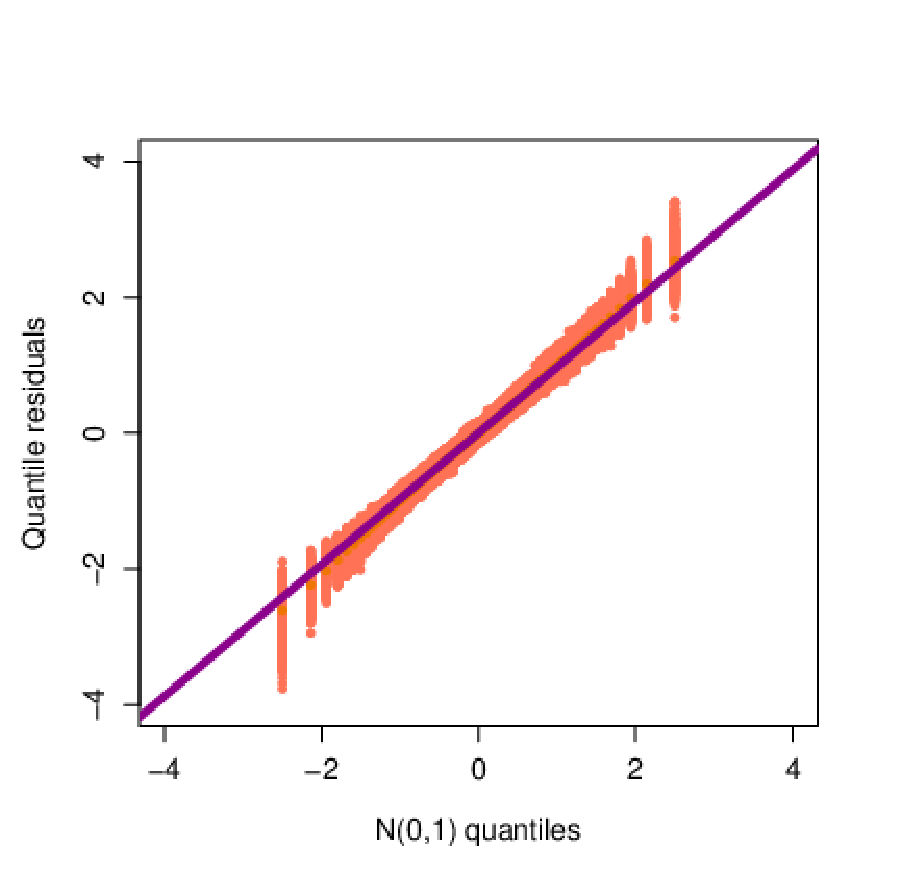
\includegraphics[width=5cm,height=5cm]{n_100_theta_0_6_alpha_0_4.eps}~
				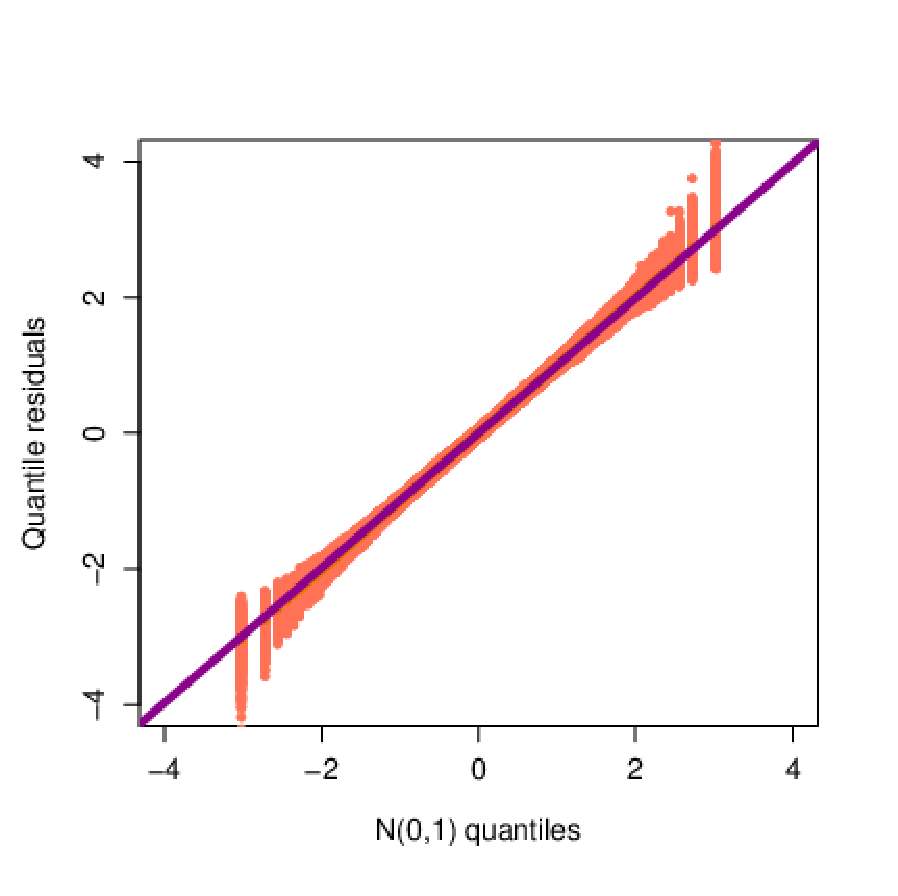
\includegraphics[width=5cm,height=5cm]{n_500_theta_0_6_alpha_0_4.eps}~
				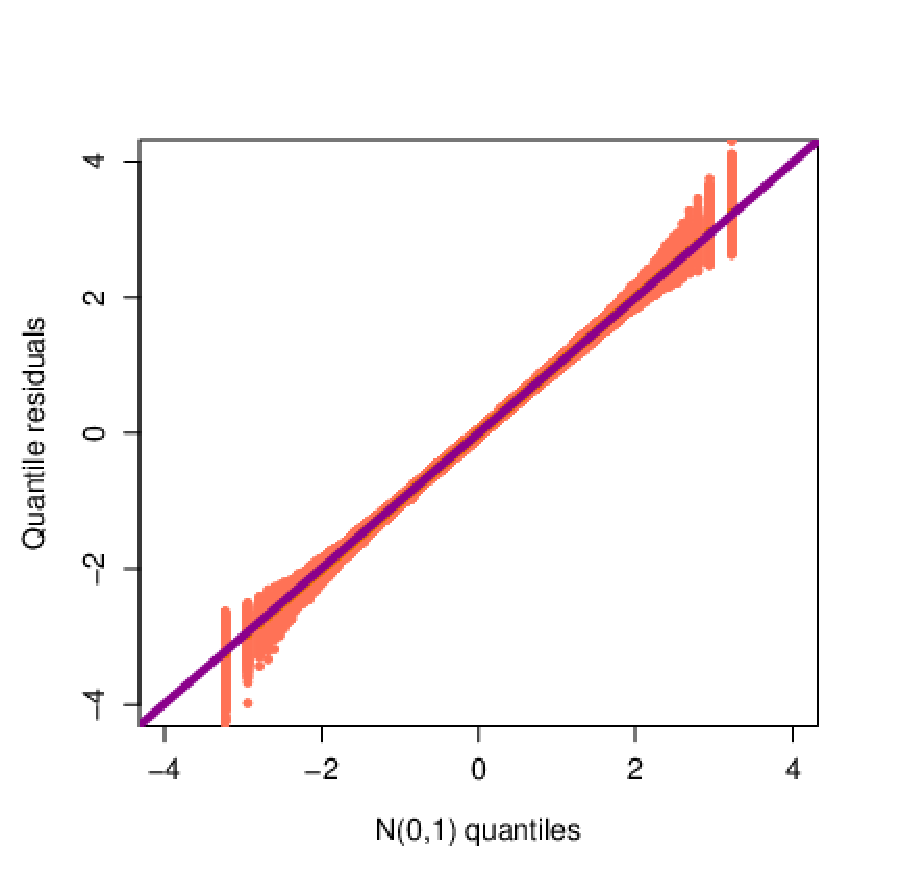
\includegraphics[width=5cm,height=5cm]{n_1000_theta_0_6_alpha_0_4.eps}
				\caption{QQ plots for scenario 1 ($\theta=0.6$ and $\alpha=0.4$). (a) $n=100$. (b) $n=500$. (c) $n = 1,000$.}\label{graf_simulacao_regressao_theta_0_6_alpha_0_4}
			\end{center}
		\end{figure}		
		
		\begin{figure}[htb!]
			\begin{center}
				(a)\hspace{4.5cm}(b)\hspace{4.5cm}(c)
				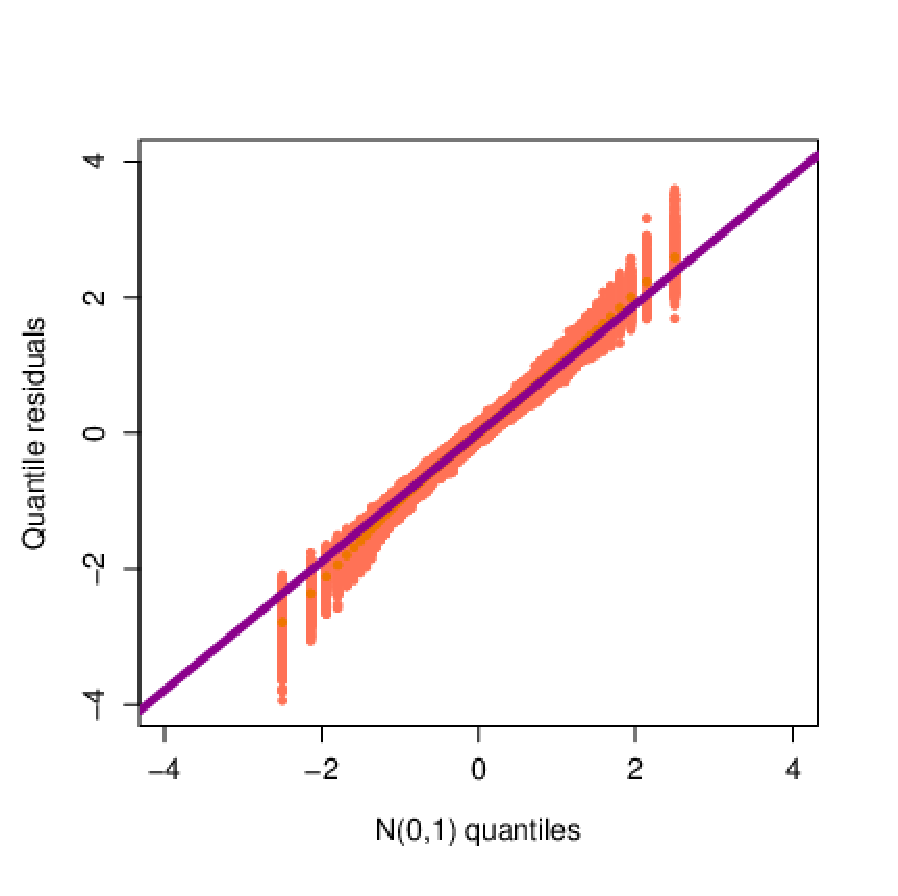
\includegraphics[width=5cm,height=5cm]{n_100_theta_0_6_alpha_1_4.eps}~
				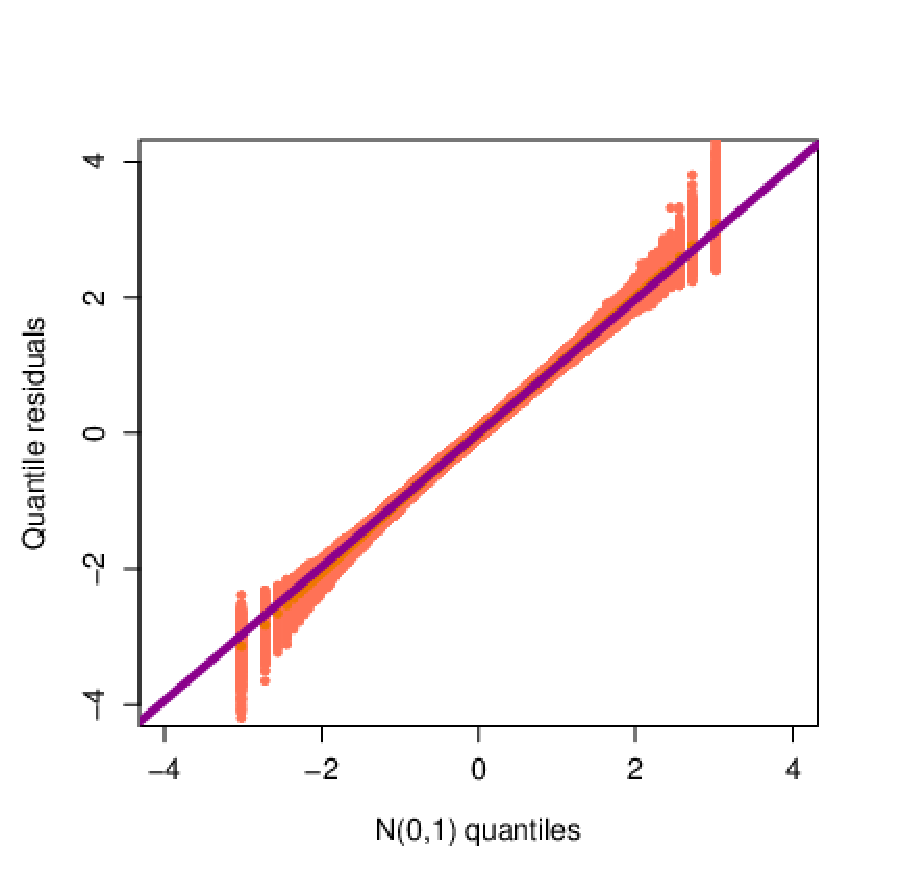
\includegraphics[width=5cm,height=5cm]{n_500_theta_0_6_alpha_1_4.eps}~
				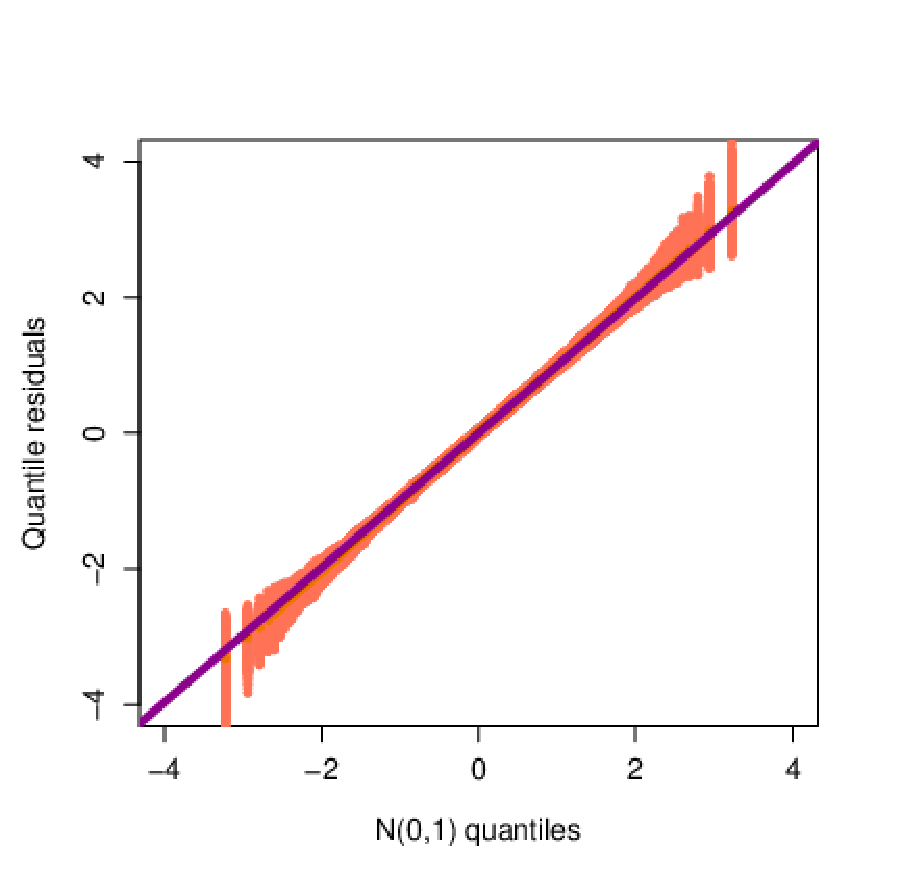
\includegraphics[width=5cm,height=5cm]{n_1000_theta_0_6_alpha_1_4.eps}
				\caption{QQ plots for scenario 2 ($\theta=0.6$ and $\alpha=1.4$). (a) $n=100$. (b) $n=500$. (c) $n = 1,000$.}\label{graf_simulacao_regressao_theta_0_6_alpha_1_4}
			\end{center}
		\end{figure}
		
		
		\begin{figure}[!htb]\small
			\begin{center}
				(a)\hspace{4.5cm}(b)\hspace{4.5cm}(c)
				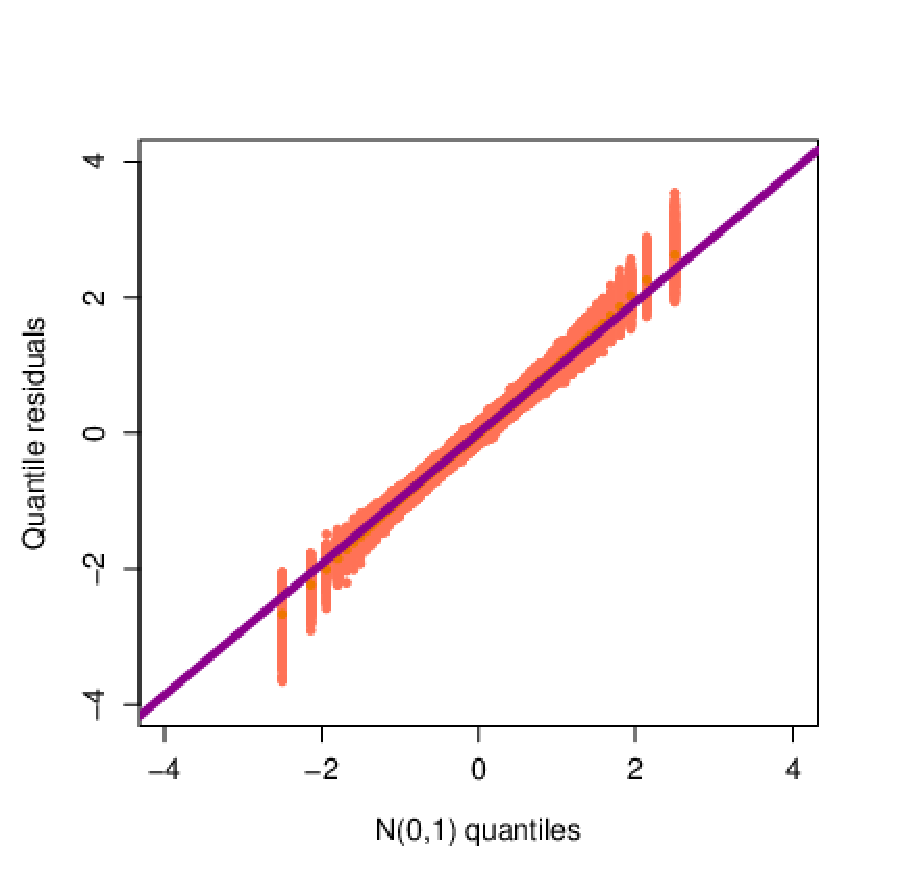
\includegraphics[width=5cm,height=5cm]{n_100_theta_1_7_alpha_0_4.eps}~
				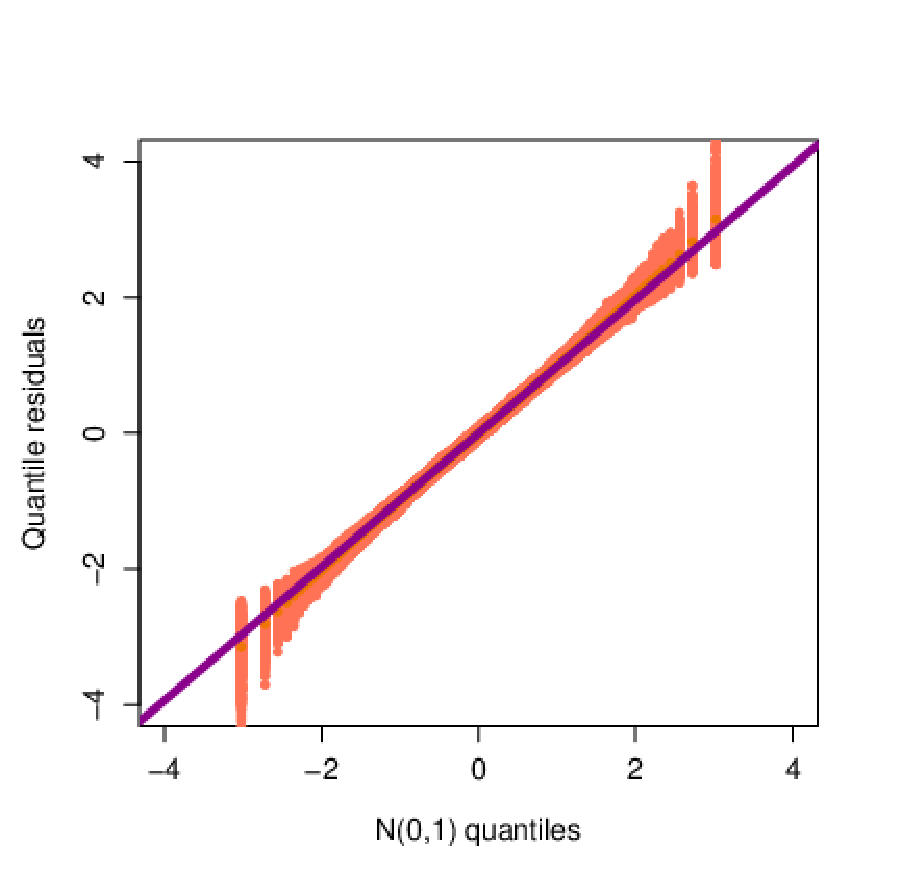
\includegraphics[width=5cm,height=5cm]{n_500_theta_1_7_alpha_0_4.eps}~
				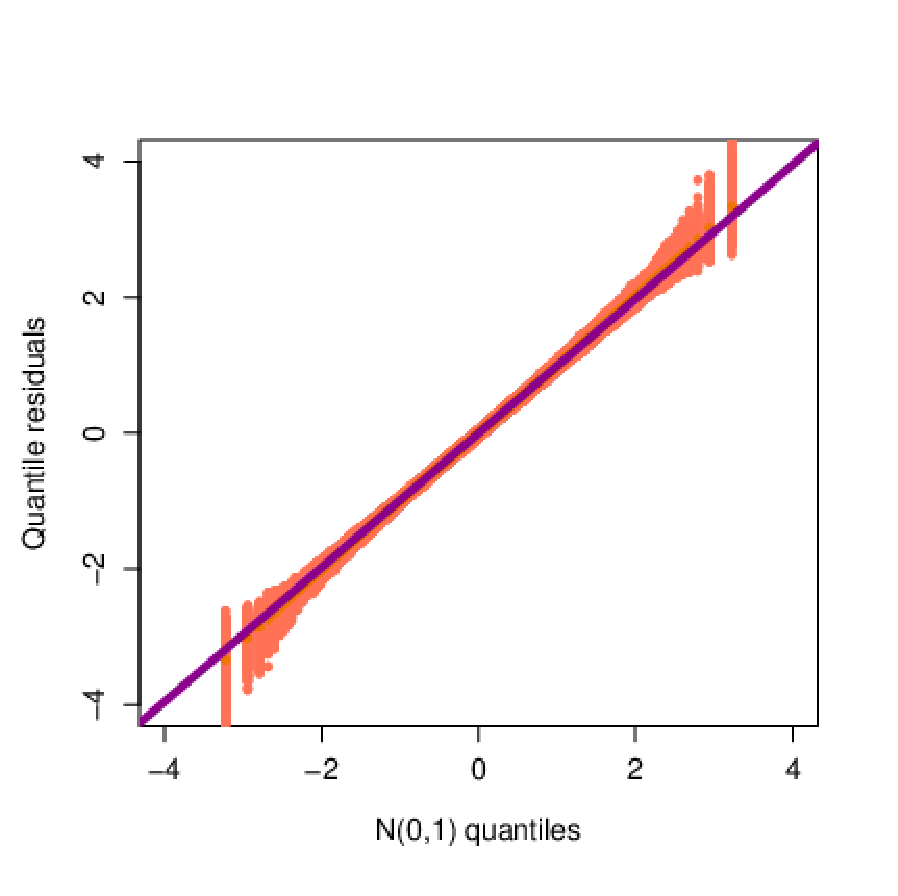
\includegraphics[width=5cm,height=5cm]{n_1000_theta_1_7_alpha_0_4.eps}
				\caption{QQ plots for scenario 3 ($\theta=1.7$ and $\alpha=0.4$). (a) $n=100$. (b) $n=500$. (c) $n = 1,000$.}\label{graf_simulacao_regressao_theta_1_7_alpha_0_4}
			\end{center}
		\end{figure}		
		\begin{figure}[!htb]\small
			\begin{center}
				(a)\hspace{4.5cm}(b)\hspace{4.5cm}(c)
				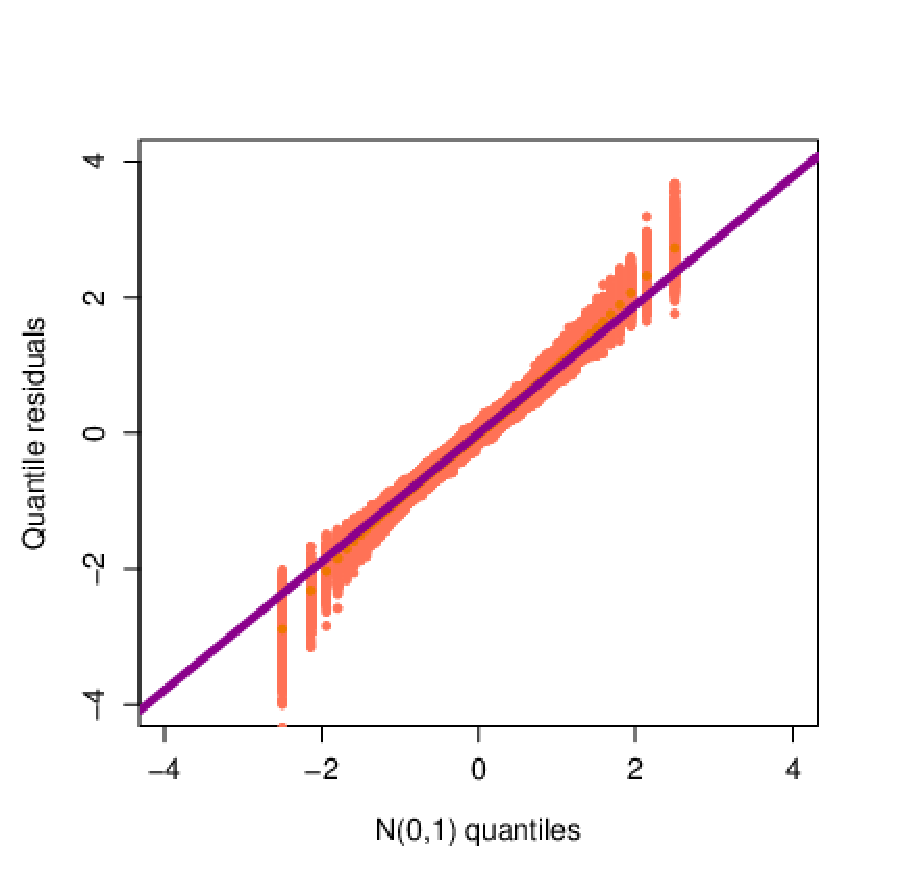
\includegraphics[width=5cm,height=5cm]{n_100_theta_1_7_alpha_1_4.eps}~
				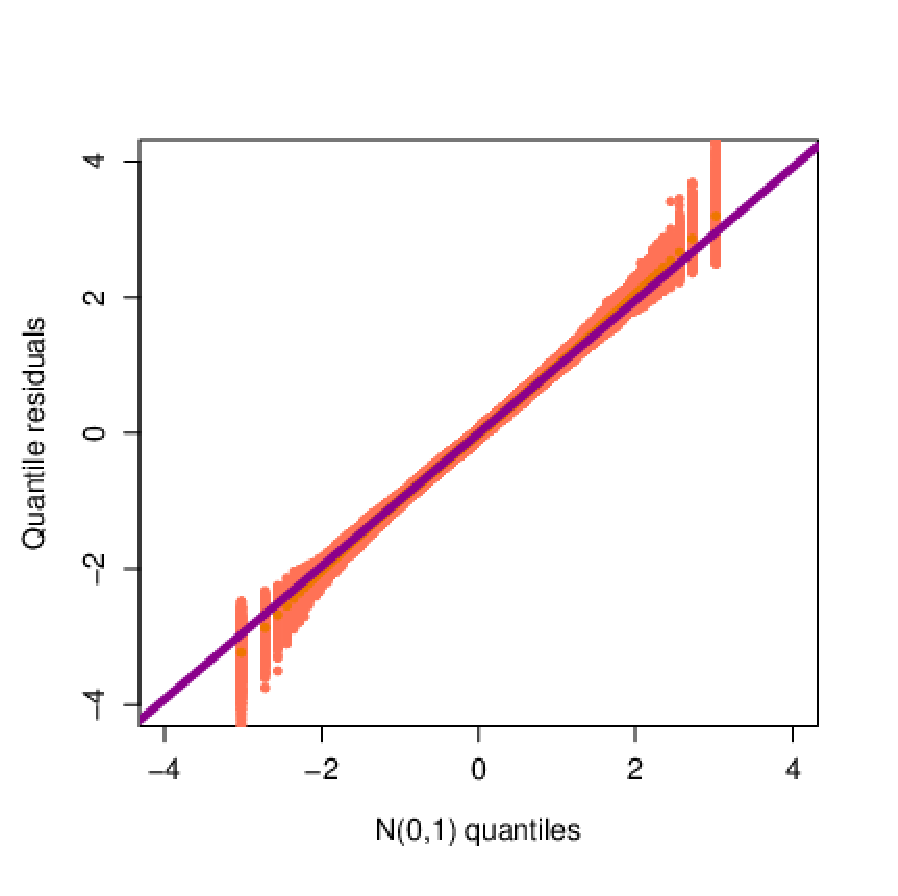
\includegraphics[width=5cm,height=5cm]{n_500_theta_1_7_alpha_1_4.eps}~
				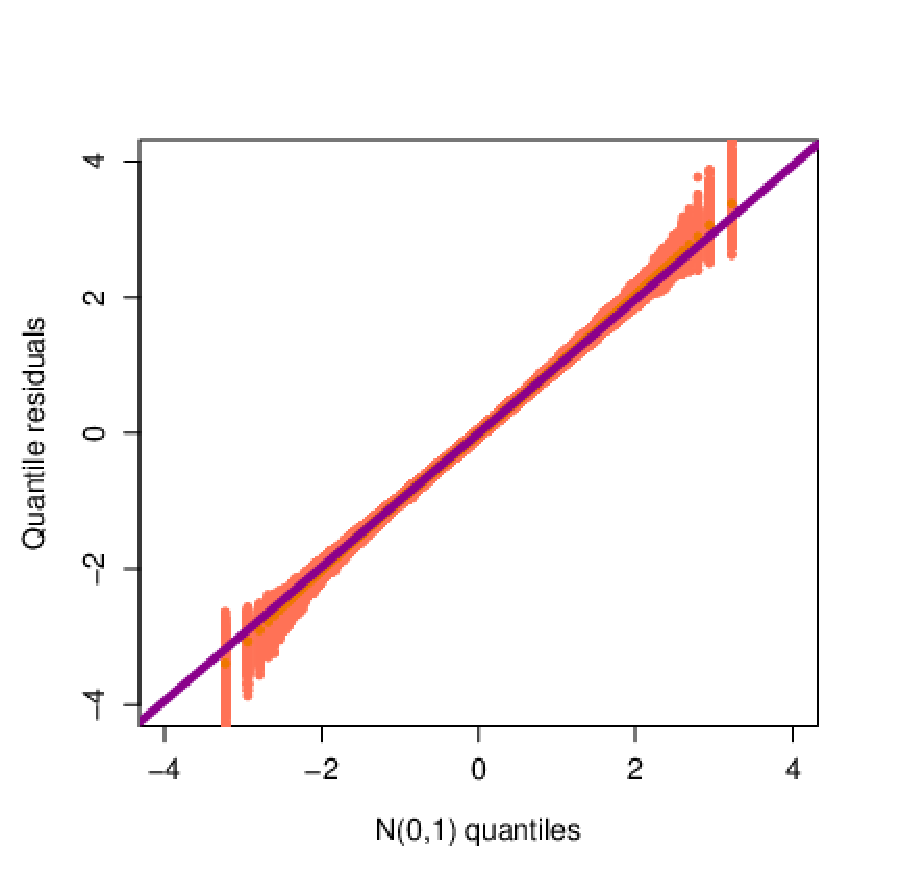
\includegraphics[width=5cm,height=5cm]{n_1000_theta_1_7_alpha_1_4.eps}
				\caption{QQ plots for scenario 4 ($\theta=1.7$ and $\alpha=1.4$). (a) $n=100$. (b) $n=500$. (c) $n = 1,000$.}\label{graf_simulacao_regressao_theta_1_7_alpha_1_4}
			\end{center}
		\end{figure}

%%%%%%%%%%%%%%%%%%%%%%%%%%%%%%%%%%%%%%%%%%%%%%%%%%%%%%%%%%%%%%%%%%%%%%%%%%%%%%%%%%%%%%	
\section{Applications}\label{applications}
The beta Weibull (BW) and Kumaraswamy Weibull (KwW) distributions have been widely
used to fit real data in the last ten years or so. We compare the MOTPW distribution with the BW and
KwW distributions since all of them have four parameters. The BW density pioneered  by \cite{Lee2007} is
\begin{eqnarray*}
f(x)=\frac{c\lambda^c}{B(a,b)}x^{c-1} {\rm exp}\{-b(\lambda
x)^c\}[1-{\rm exp}\{-(\lambda x)^c\}]^{a-1},\,\,x>0,
\end{eqnarray*}
where all parameters are positive.

The KwW density introduced by \cite{Cord2011} has the form
\begin{eqnarray*}
f(x)= a\,b\,c\,\lambda^cx^{c-1}\exp\{-(\lambda x)^c\} [1 -\exp
\{-(\lambda x)^c\}]^{a-1}\{1-[1-\exp\{-(\lambda x)^c\}]^{a}\}^{b-1},\,\, x>0,
\end{eqnarray*}
where all parameters are positive.



\subsection{Application 1: Hourly dollar wage data}\label{applications1}

The first application refers to hourly dollar wages for $n=534$ US workers.
These data are obtained from the {\it SemiPar} package \citep{wand2005semipar}.
Table \ref{EMV_salario_} lists the estimates, standard errors (SEs) in
parentheses, and three classical statistics. The lowest values
of these measures reveal that the MOTPW is the best model. Next, the likelihood ratio (LR) statistic for
comparing the MOTPW and TPW models is $6.159\,(\mbox{p-value} < 0.013)$ which supports the wider distribution.

Figure \ref{dens_salario}a shows the histogram and the estimated MOTPW density. Figure \ref{dens_salario}b
provides the empirical function and estimated MOTPW cdf, thus revealing that this distribution is appropriate
for these data.

\begin{table}[htb!]
	\centering{\caption{Results for hourly dollar wage data.}\label{EMV_salario_}}
	\vspace*{0.3cm}
	\begin{tabular}{ccccc|ccc}
		\hline
		Model      &$\log(\lambda)$      & $\log(\beta)$ & $\theta$  & $\alpha$ &AIC      &BIC     &GD    \\
		\hline
		{\bf MOTPW}     &-2.720  &0.694   &11.210   &0.019 &{\bf 3031.288}  &{\bf 3048.410} &{\bf 3023.288}\\
		&(0.141)  &(0.085) &(3.020) &(0.007) &&&\\
		TPW       &0.248   &-0.541  &31.100   &(-)        &3035.448  &3048.289  &3029.448\\
		          &(0.444) &(0.112) &(12.540) &(-)      &&&      \\
        \hline
        Model      &$\log(\lambda)$      &$a$ & $b$  &$\log(c)$ &AIC      &BIC     &GD    \\
		\hline
		KwW       &-0.601  &12.124  &0.317   &0.060    &3034.039  &3051.160  &3026.039\\
		          &(0.023) &(0.802) &(0.013) &(0.014)  &          &          &        \\
		BW        &-5.453  &2.327   &126.000 &0.216    &3084.086  &3101.208  &3076.086\\
		          &(0.020) &(0.067) &(0.009) &(0.007)  &          &          &        \\
		\hline
		\end{tabular}
		\end{table}	
%		\begin{table}[htb!]
%		\centering {\caption{Medidas de seleção de modelos para os dados de salário em dólares por hora.}
%			\label{goodness:salario}}
%		\vspace*{0.3cm}
%		\begin{tabular}{cccc}
%		\hline
%		Model    &AIC      &BIC     &GD\\
%		\hline
%		{\bf MOTPW} &{\bf 3031.288}  &{\bf 3048.410} &{\bf 3023.288}\\
%		TPW         &3035.448  &3048.289  &3029.448\\
%		\hline
%		\end{tabular}
%		\end{table}
%Na Tabela \ref{rv_salario} s{\~a}o exibidas as estat{\'i}sticas de LR para comparar a distribui{\c{c}}{\~a}o aninhada. Portanto, rejeita-se a hip{\'o}tese nula a favor da distribui{\c{c}}{\~a}o MOTPW.
%		
%		\begin{table}[htb!]
%		\centering {\caption{Testes LR para os dados de salário em dólares por hora.\label{rv_salario}}\vspace*{0.3cm}
%			\begin{tabular}{c|c|c|c}
%			\hline Models & Hypothesis  &LR statistic & p-value  \\
%			\hline
%			MOTPW vs TPW & $H_{0}:\alpha=1$ vs $H_{1}: H_{0}\,\mbox{is\,false}$    &6.159    &0.013\\
%			\hline
%		\end{tabular}}
%	\end{table}
%	Observe que, o gr{\'a}fico da Figura \ref{dens_salario}(a) revela o histograma de de salário em dólares por hora, note que a curva da densidade estimada da distribui{\c{c}}ão proposta se aproxima mais do histograma dos dados. J{\'a} no gr{\'a}fico da Figura \ref{dens_salario}(b) a qualidade do ajuste marginal {\'e} comprovada, pois, a cdf estimada da distribuição MOTPW fica mais pr{\'o}xima da cdf emp{\'i}rica dos dados em rela{\c{c}}{\~a}o ao modelo TPW, portanto, a distribui{\c{c}}{\~a}o MOTPW {\'e} uma boa op{\c{c}}{\~a}o para modelar esses dados.	
	\begin{figure}[!htb]
		\begin{center}
			(a)\hspace{5cm}(b)\\					
			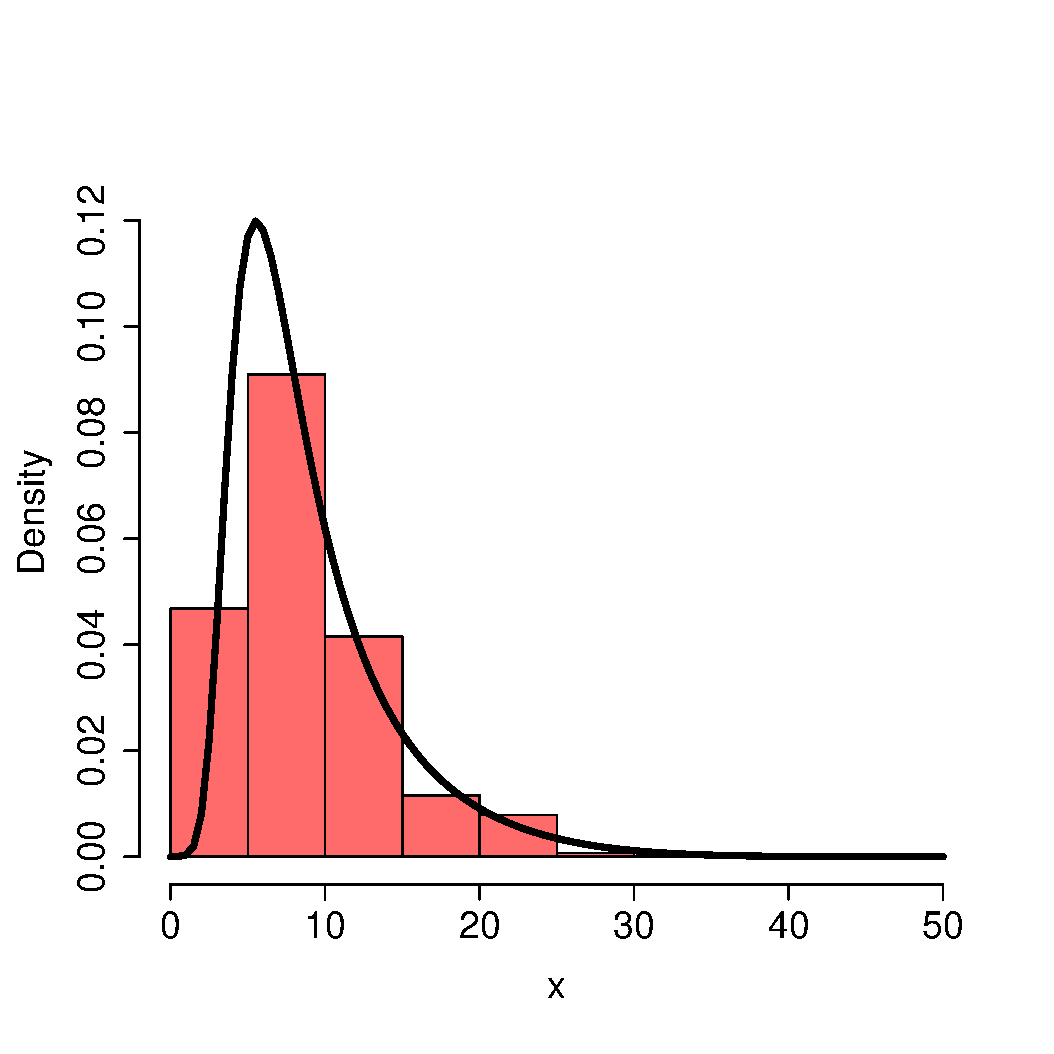
\includegraphics[width=5.5cm,height=5.5cm]{Ajuste_marginal_dens_estimada.eps}
			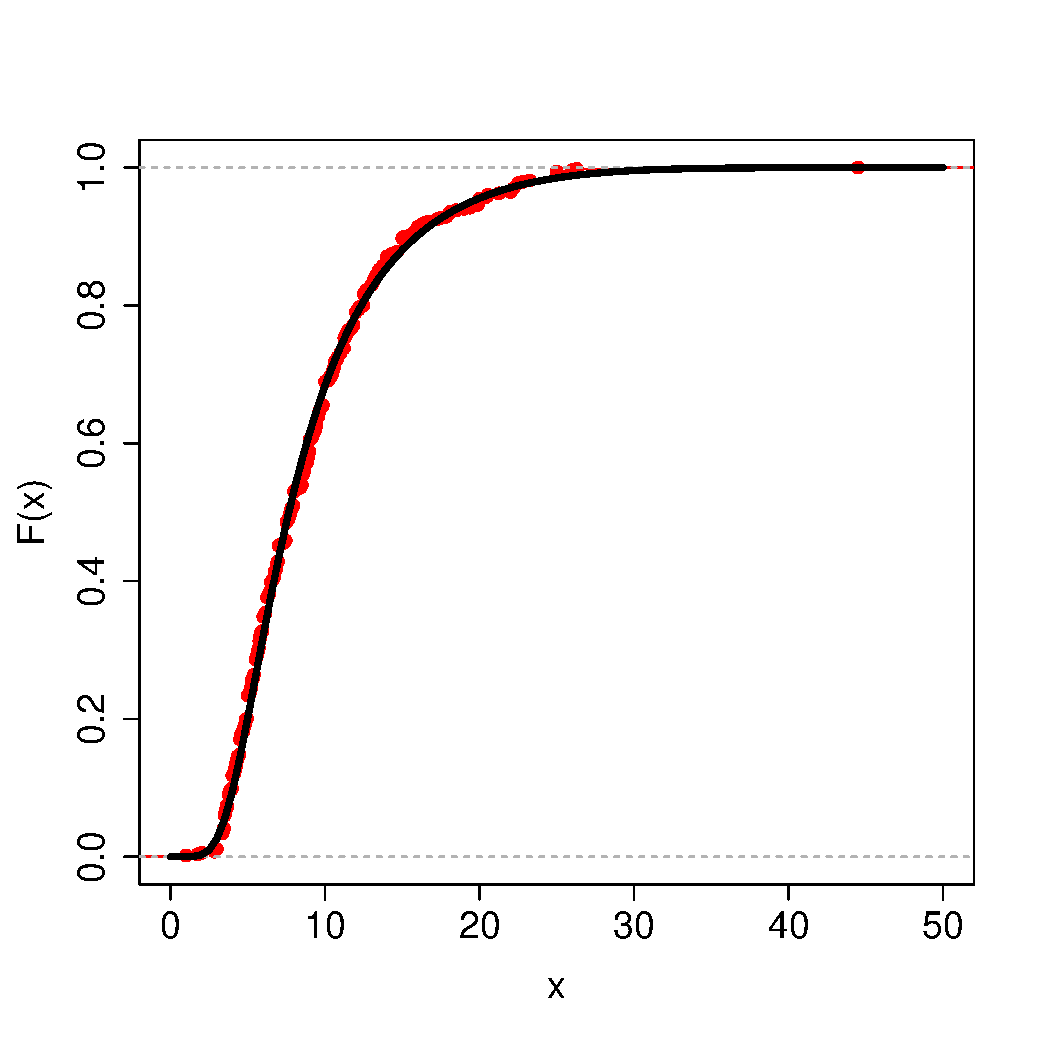
\includegraphics[width=5.5cm,height=5.5cm]{Ajuste_marginal_acum_estimada.eps}
			\caption{(a) Estimated MOTPW pdf. (b) Estimated MOTPW cdf and the empirical cdf.\label{dens_salario}}
		\end{center}
	\end{figure}
	
	
%%%%%%%%Modelo de regressão%%%%%%%%%%%%%%%%%%%%%%%%%%%%%%%%%%%%%%%%%%%%%%%%%%%%%


\subsection{Application 2: Diabetes data.}\label{applications2}
	
We consider two variables from the data reported by \cite{Reaven1979}: the response $x_i$ is the relative weight defined by the ratio between
the actual weight and the expected weight (given the person's height), and the explanatory variable $v_{i1}$ indicates the diagnostic group (0 =normal, 1=
chemical diabetes, 2 = overt diabetes). The diagnostic group has three levels and then we have two dummy variables $(d_ {ij})$ (for $i= 1,\ldots,145$
and $j= 1,2$). The objective is to know what are the relations among the relative weight and the levels of the diagnostic group.

The systematic components for the MOTPW regression are
$$\lambda_i =\exp\left(\eta_{10}+\eta_{11}d_{i1}+\eta_{12}d_{i2}\right)\quad \text{and}
\quad \beta_i =\exp\left(\eta_{20}+\eta_{21}d_{i1}+\eta_{22}d_{i2}\right),\quad i=1,\ldots,145.$$
	
The measures for the fitted regressions are reported in Table \ref{goodness:regressao_aplicacao_2}.
Clearly, the MOTPW is the best regression for these data.
	
	\begin{table}[htb!]
		\centering {\caption{Measures for diabetes data.}\label{goodness:regressao_aplicacao_2}}
		\vspace*{0.3cm}
		\begin{tabular}{cccc}
			\hline
			Model &AIC &BIC  &GD  \\
			\hline
			{\bf MOTPW} &{\bf -194.316}  &{\bf -170.502}  &{\bf -210.316}\\			
			TPW         &-191.726        &-170.889        &-205.726\\			
			KwW         &-188.769        &-164.955        &-204.769\\			
			BW          &-185.607        &-161.793        &-201.607\\			
			\hline
		\end{tabular}
	\end{table}
Table \ref{EMV_regressao_aplicacao_2} provides the estimates, SEs and $p$-values for the best regression.
	\begin{table}[htb!]
		\centering {\caption{Results for diabetes data.}
			\label{EMV_regressao_aplicacao_2}}
		\vspace*{0.3cm}
		\begin{tabular}{cccc}
			\hline
			Parameter     & Estimate   &SE      &p-Value\\
			\hline
			${\eta}_{10}$   &0.065  &0.093  &0.489\\
			${\eta}_{11}$   &-0.119 &0.036  &0.001\\
			${\eta}_{12}$   &-0.049 &0.028  &0.082\\
			\hline
			${\eta}_{20}$   &1.719 &0.245 &$<$0.001\\
			${\eta}_{21}$   &0.373 &0.140 &0.009\\
			${\eta}_{22}$   &0.131 &0.141 &0.355\\
			\hline
			${\theta}$      &12.401&8.866 &\\
			${\alpha}$      &0.095 &0.079 &\\		
			\hline
		\end{tabular}
	\end{table}

We note that the co-variable $d_{i1}$ is significant and  $d_{i2}$ is not. So, there is a real difference between
normal and chemical diabetes groups in relation to relative weight and no difference between normal and overt
diabetes groups to relative weight. The same findings can be seen in Figure \ref{diferenca}.

The LR statistic to compare the MOTPW and TPW regressions is $w=4.590$ ($p$-value=0.032) that indicates
that the fist regression is superior to the second regression to these data in terms of model fitting.


The plot of the residuals reported in Figure \ref{graf_res_quantile_aplicacao_2}a does not detect outliers and departures
from the general assumptions. The worm plot \citep{Buuren2001} of the residuals in Figure \ref{graf_res_quantile_aplicacao_2}b
and the QQ plot displayed in Figure \ref{graf_res_quantile_aplicacao_2}c show the adequacy of the MOTPW regression
for the current data.
		
		\begin{figure}[!htb]
			\begin{center}
				(a)\hspace{4.5cm}(b)\hspace{4.5cm}(c)\\					
				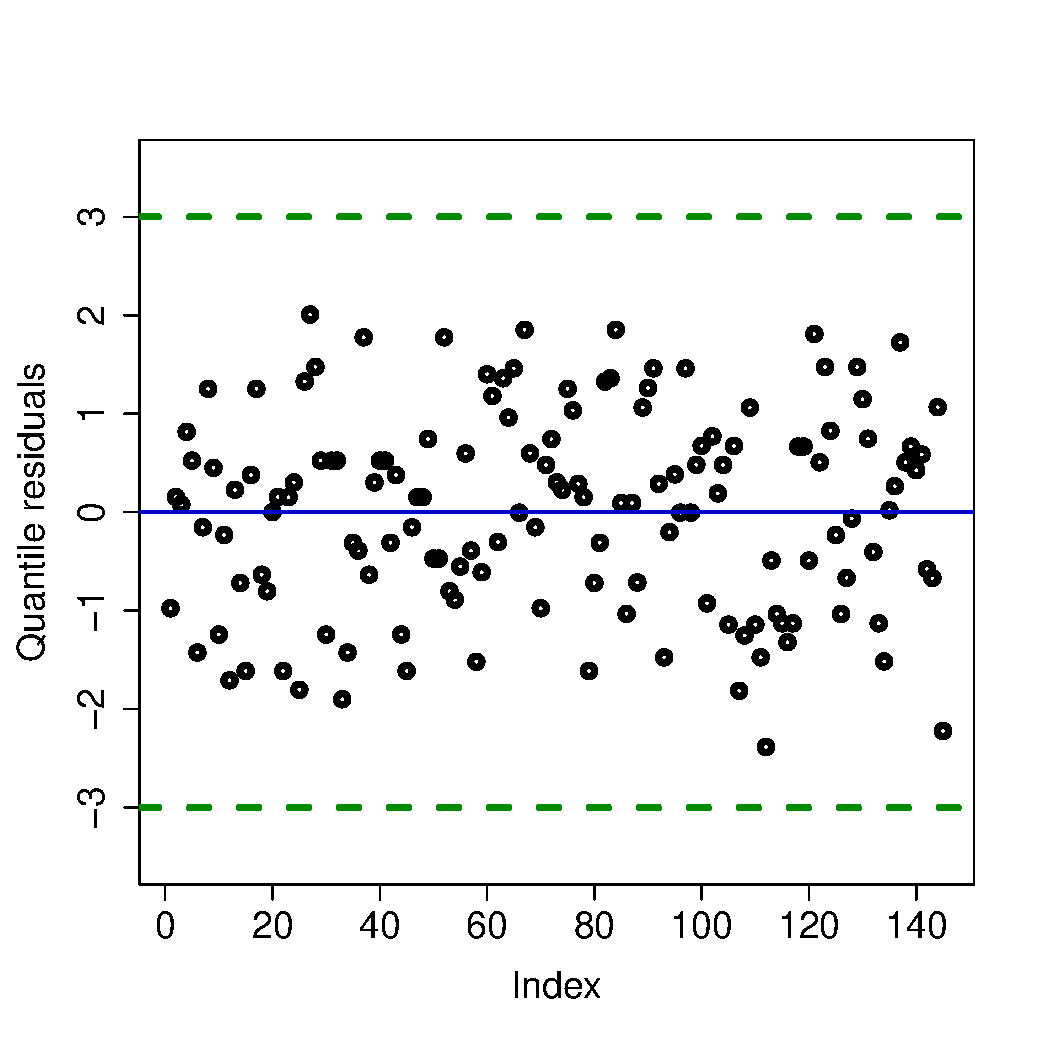
\includegraphics[width=5cm,height=5cm]{Res_quantilico_vs_indices.eps}
				~~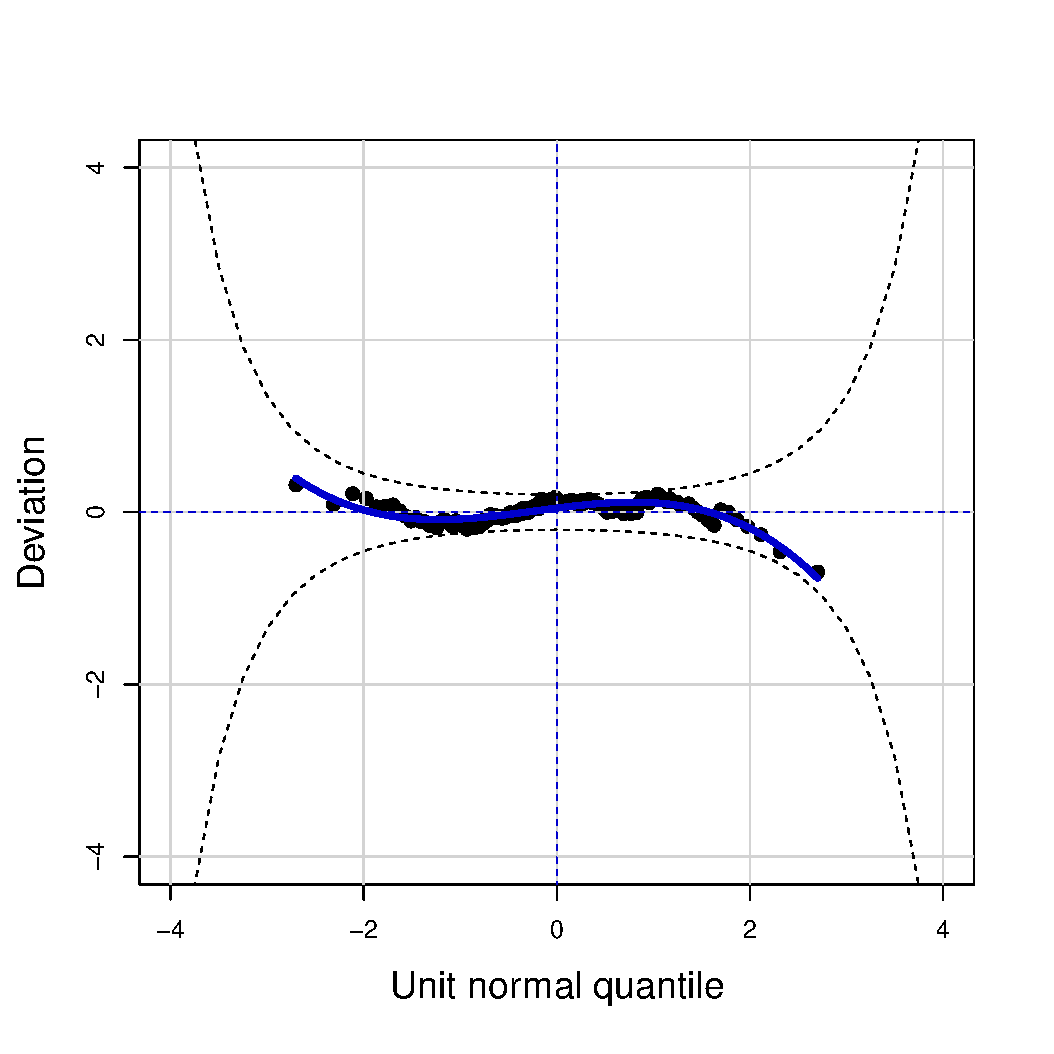
\includegraphics[width=5cm,height=5cm]{wormplot.eps}
                ~~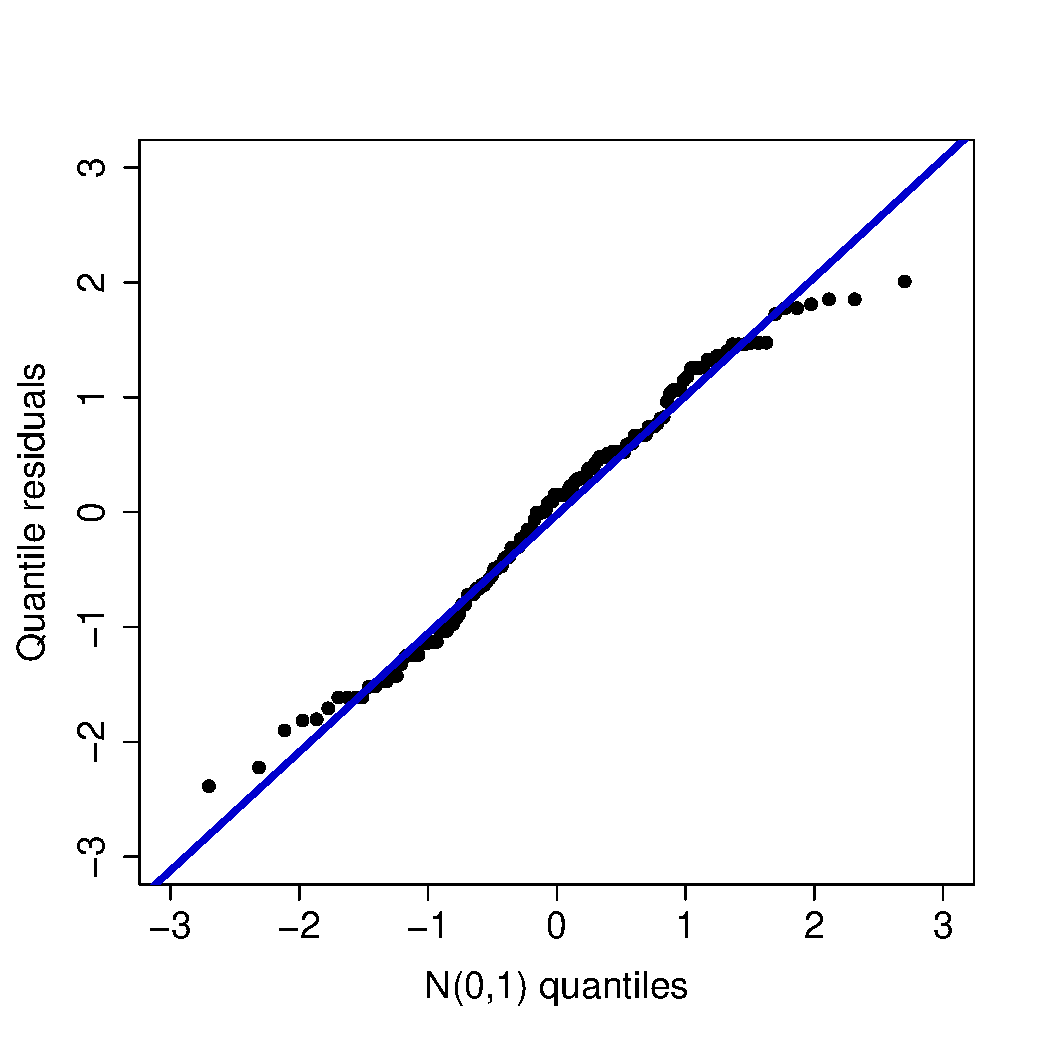
\includegraphics[width=5cm,height=5cm]{qqnorm.eps}
				\caption{(a) Residual plot. (b) Worm plots. (c) QQ plot.}
				\label{graf_res_quantile_aplicacao_2}
			\end{center}
		\end{figure}

A graphical comparison from the estimated cdfs in Figure \ref{diferenca} also supports the regression analysis.
		\begin{figure}[!htb]
			\begin{center}
				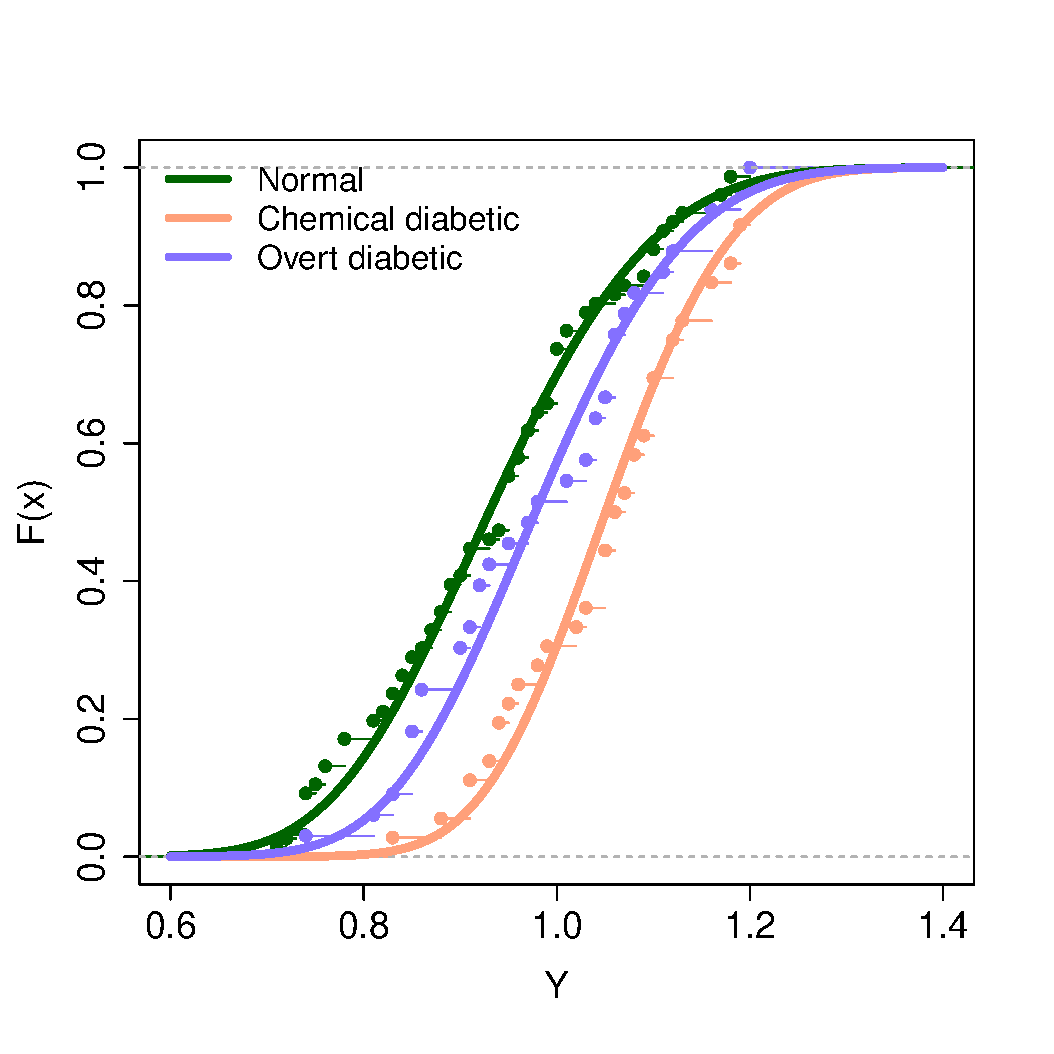
\includegraphics[width=5.5cm,height=5.5cm]{diferenca.eps}
				\caption{Estimated cdf and the empirical cdf.}
				\label{diferenca}
			\end{center}
		\end{figure}


\section{Concluding Remarks}\label{conclusions}

We define two flexible Marshall--Olkin--Power-Series (MOPS) families of continuous distributions which can be very useful to fit real data.
They are obtained by combining the Marshall--Olkin class \citep{MarshallOlkin1997} and the power series
distribution. Hundreds of continuous distributions can be easily formulated from the two families. We discuss some special distributions and maximum
likelihood estimation. We introduce the {\it Marshall--Olkin Truncated Poisson Weibull} regression associated with one of the families.
Some mathematical properties of these families are presented. The utility of the proposed models is proved empirically in two
applications.


\section*{Acknowledgments}

We gratefully acknowledge from CNPq and CAPES, Brazil.



{\small
\bibliographystyle{chicago}	
\begin{thebibliography}{}
\renewcommand{\itemsep}{0pt}

% Reference 4
\bibitem[\protect\citeauthoryear{Buuren and Fredriks}{2001}]{Buuren2001}
BUUREN SV AND FREDRIKS M. 2001.
Worm plot: a simple diagnostic device for modelling growth reference curves. {\em Statistics in Medicine}, {\bf 20}, 1259--1277.

% Reference 8
\bibitem[\protect\citeauthoryear{Cordeiro and Castro}{2011}]{Cord2011}
CORDEIRO GM AND DE CASTRO M. 2011.
A new family of generalized distributions. {\em Journal of Statistical Computation and Simulation}, {\bf 81}, 883--898.

% Reference 11
\bibitem[\protect\citeauthoryear{Dunn and Smyth}{1996}]{Dunn1996}
DUNN PK AND SMYTH GK. 1996.
Randomized quantile residuals. {\em Journal of Computational and Graphical Statistics}, {\bf 5}, 236--244.

\bibitem[\protect\citeauthoryear{Lee et al.}{2007}]{Lee2007}
LEE C, FAMOYE F AND OLUMOLADE O. 2007.
Beta Weibull distribution: Some properties
and applications to censored data. {\em Journal of Modern Applied Statistical Methods}, {\bf 6}, 173-186.

% Reference 26
\bibitem[\protect\citeauthoryear{Marshall and Olkin}{1997}]{MarshallOlkin1997}
MARSHALL AW AND OLKIN I. 1997.
A new method for adding a parameter to a family of distributions with application to the exponential and Weibull families. {\em Biometrika}, {\bf 84}, 641--652.

\bibitem[\protect\citeauthoryear{R Core Team}{2021}]{rlang} R Core Team (2021). R: A language and environment for statistical computing. R Foundation for Statistical Computing, Vienna, Austria. URL https://www.R-project.org/.

% Reference 34
\bibitem[\protect\citeauthoryear{Reaven and Miller}{1979}]{Reaven1979}
REAVEN GM AND MILLER RG 1979.
An attempt to define the nature of chemical diabetes using a multidimensional analysis. {\em Diabetologia}, {\bf 16}, 17--24.

% Reference 38
\bibitem[\protect\citeauthoryear{Stasinopoulos et al.}{2007}]{Stasinopoulos2007}
STASINOPOULOS DM AND RIGBY RA. 2007.
Generalized additive models for location scale and shape (GAMLSS) in R. {\em Journal of Statistical Software}, {\bf 23}, 1--46.

% Reference 39
\bibitem[\protect\citeauthoryear{Wand et al.}{2005}]{wand2005semipar}
WAND MP, COULL BA, FRENCH JL, GANGULI B, KAMMANN EE, STAUDENMAYER J AND ZANOBETTI A. 2005.
SemiPar 1.0. R package. {\em URL: http://cran. r-project. org}.

\bibitem[\protect\citeauthoryear{Tahir and Nadarajah}{2015}]{Tahir2015}
TAHIR M AND NADARAJAH S. 2015.
Parameter induction in continuous univariate distributions: Well established G-classes.
{\it Annals of the Brazilaian Academy of Sciences}, {\bf 87}, 539--568.



\end{thebibliography}


\end{document}
